\documentclass[12pt,a4paper, openany]{report}

%\documentclass[12pt,a4paper, openany]{article}
\usepackage[utf8]{inputenc}
%\usepackage[T1]{fontenc}

\usepackage[T1]{fontenc}
\usepackage{graphicx}
\usepackage{mathtools}
\usepackage{amssymb}
\usepackage{amsthm}

\usepackage{amsmath}
\usepackage{amsfonts}
\usepackage{amssymb}
\usepackage{thmtools}
\usepackage{xcolor}
\usepackage{color}
\usepackage{shorttoc}
\usepackage{nameref}
\usepackage[colorlinks=true,urlcolor=blue]{hyperref}
\usepackage[french]{babel}
\usepackage{setspace}
%\usepackage[margin=1in]{geometry}
\usepackage{tikz}
\usepackage{lmodern}
\usepackage{tocloft}
\usepackage[a4paper]{geometry}
% Packages nécessaires
\usepackage{fancyhdr}
\usepackage{minitoc}
\usepackage{titlesec}
\usepackage{lipsum}  % Pour générer du texte d'exemple



% Configuration des hyperliens
\hypersetup{
	colorlinks=true,
	linkcolor=blue,
	filecolor=magenta,      
	urlcolor=cyan,
}

\definecolor{GREEN}{rgb}{0.0, 1.0, 0.0}
%\definecolor{green!30!blue}{rgb}{0.0, 1.0, 0.0}
\definecolor{BLUE}{rgb}{0.0, 0.0, 1.0}


\usepackage{booktabs,tabularx,longtable,supertabular,colortbl,lettrine,multicol, multirow}
\usepackage{amsmath,amssymb,amsfonts,frcursive,pifont,mathrsfs,calligra,palatino,frcursive}
\usepackage{ulem, tikz, pifont, fancyvrb, alltt,rotating,pgf}
\usepackage{graphicx,type1cm,eso-pic,color,carolmin,diagbox,framed,fancyhdr,diagbox,fancybox}

% Configuration de la table des matières
\renewcommand{\cftchapfont}{\bfseries}
\renewcommand{\cftsecfont}{\normalfont}
\renewcommand{\cftchappagefont}{\bfseries}
\renewcommand{\cftsecpagefont}{\normalfont}
\renewcommand{\cftchapleader}{\cftdotfill{\cftdotsep}}

% Configuration des en-têtes et pieds de page
\pagestyle{fancy}
\fancyhf{}
\fancyhead[L]{\leftmark}
\fancyhead[R]{\thepage}
\renewcommand{\headrulewidth}{1.5pt}
\renewcommand{\footrulewidth}{1.5pt}
\fancypagestyle{vide}{
	\pagestyle{fancy}
	\fancyhf{} % efface tout ce qu'il y avait avant
	\fancyfoot[CO]{}
	\fancyfoot[CE]{}
	\renewcommand{\footrulewidth}{0pt}
	\renewcommand{\headrulewidth}{0pt}
}

% Configuration des titres
\titleformat{\chapter}[hang]
{\normalfont\huge\bfseries}{\thechapter.}{1em}{}
\titleformat{\section}[hang]
{\normalfont\Large\bfseries}{\thesection}{1em}{}
\titleformat{\subsection}[hang]
{\normalfont\large\bfseries}{\thesubsection}{1em}{}



\makeatletter
\newcommand{\thechapterwords}
{ \ifcase \thechapter\or 1 \or 2 \or 3 \or 4\or 5\or
	6\or 7\or 8 \or 9  \or 10 \or 11\or 12\or
	13\or 14\or 15 \or 16 \or17\fi}
\def\thickhrulefill{\leavevmode \leaders \hrule height 1.7ex \hfill \kern \z@}
\def\@makechapterhead#1{%
	%     \vspace*{15\p@}%
	\begin{tikzpicture}[remember picture, overlay]
		\begin{scope}[shift={(current page.south west)},shift={(3.7, -0.5)},scale=1]
			\filldraw[fill=gray, opacity=1] (3, 27.8) rectangle (15.2, 28.7);
			\draw (0.2,28.2) node {\sl\cminfamily\Huge\@chapapp{} \thechapter};
		\end{scope}
	\end{tikzpicture}%\hspace{1cm}
	{\parindent \z@ \centering \reset@font
		% \thickhrulefill\quad
		%\slshape {\color{black!50!red}\@chapapp{} \thechapterwords}
		%         \quad \thickhrulefill
		%\par\nobreak
		%\vspace*{5\p@}%
		\interlinepenalty\@M
		%{\color{blue!10!blue}\hrule height 1.5ex}
		%\vspace*{15\p@}%
		\Huge\sl \bfseries #1\par\nobreak
		\par
		\vspace*{15\p@}%
		{\color{blue!40!blue}\hrule}
		\vskip 60\p@
		%\vskip 100\p@
}}


\definecolor{mygray}{gray}{.80}
\def\thickhrulefillm{\leavevmode \leaders \hrule height 3.5ex \hfill \kern \z@}
\def\@makeschapterhead#1{%
	{\parindent \z@ \centering \reset@font
		%         \thickhrulefill
		{\color{mygray}\thickhrulefillm}
		%         \par\nobreak
		%         \vspace*{15\p@}%
		%         \interlinepenalty\@M
		%         \hrule
		%         \vspace*{15\p@}%
		\sl\Huge \bfseries #1\par\nobreak
		\par
		\vspace*{1\p@}%
		\hrule
		\vskip 40\p@
		%\vskip 100\p@
}}
\linespread{1.5}


\begin{document}
	\newgeometry{margin=-0.3cm}
	
	\begin{center}
		\begin{tikzpicture}
			\draw[thick] (-10.5,-15) rectangle (10.6,15);
			\fill[blue!80!gray!30] (-10.5,-15) rectangle (-3,15);
			{\node at (3.7,13)[]{\LARGE \textbf{{{\textsf{INSTITUT DE MATHÉMATIQUES}}}}};
			\node at (3.5,11.4)[]{\LARGE \textbf{{{\textsf{ET DE SCIENCES PHYSIQUES}}}}};}
			
			%\node at (3.75,10)[]{\textcolor{blue}{Centre d’Excellence Africain en Sciences Mathématiques et Applications}};
			\node at (3.5,9)[]{{\textit{\textbf{Adresse mail :} \textcolor{blue}{secretariat@imsp-uac.org}}}};
			
			\draw[line width=0.4mm] (-2.7,8) -- (10.6,8);
			
			\node at (-7.25,8)[]{{\sf \textbf{\textcolor{white}{UNIVERSITE D’ABOMEY}}}};
			\node at (-7.25,7.2)[]{{\sf \textbf{\textcolor{white}{CALAVI (BENIN)}}}};
			
			\node at (-6.7,-4.5)[]{{\sf \textbf{\textcolor{white}{ THE ABDUS SALAM }}}};
			\node at (-6.7,-5.2)[]{{\sf \textbf{\textcolor{white}{ INTERNATIONAL CENTRE FOR }}}};
			\node at (-6.7,-6)[]{{\sf \textbf{\textcolor{white}{ THEORETICAL PHYSICS (ITALY)}}}};
			
			\node at (-6.7,-11.3)[]{
\includegraphics[width=3.5cm]{images/imsp}};
			
			\node at (-6.7,1.5)[]{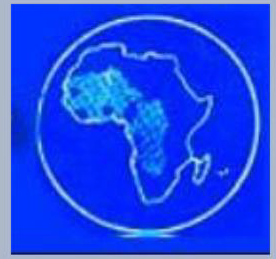
\includegraphics[width=3.7cm]{images/om}};
			
			\node at (3.5,6.9)[]{\huge \textbf{\textsf{Mémoire}}};
			\node at (3.5,5.9)[]{ \textbf{\textsf{MÉMOIRE DE MASTER 2}}};
			
			\node at (3.5,4.8)[]{{\large \textbf{\textrm{Filière : PHYSIQUE-THÉORIQUE}}}};
			
			\draw[line width=0.6mm] (-2.7,3.5) -- (10.6,3.5);
			\fill[white] (2.8,3) rectangle (5,4);
			\node at (3.8,3.55)[]{{\Large \textbf{\textsf{Thème }}}};
			\node at (3.5,2.5)[]{ {\large\centering \textbf{\textrm{\textcolor{blue}{Méthodes modernes de quantification, théorie}}}}};
			\node at (3.5,1.5)[]{ {\large\centering\textbf{\textrm{\textcolor{blue}{ ModMax et les oscillateurs harmoniques.}}}}};
			\draw[line width=0.6mm] (-2.7,0.5) -- (10.6,0.5);
			
			\node at (3.5,-0.5)[]{\large \textbf{\underline{Rédigé par :}}};
			
			\node at (3.5,-1.5)[]{{\large {BANI \:Orou Adam}}};
			\node at (3.5,-2.5)[]{\large \textit{\textbf{Adresse email :} \textcolor{blue}{baniorouadam@gmail.com}}};
		%	\node at (3.5,-3.5)[]{{\large {Et}}};
			
		%	\node at (3.5,-4.5)[]{{\large {MAMA\:Abdou Raoufou}}};
		%	\node at (3.5,-5.5)[]{\large \textit{\textbf{Adresse email :} \textcolor{blue}{mamaabdouraoufou68@gmail.com}}};
			
			%\node at (3.5,-5.5)[]{{\textit{\large IMSP-BENIN, MASTER PHYSIQUE-THÉORIQUE}}};
			
			%\node at (3.5,-3.5)[]{\large \textit{\textbf{Adresse email :} \textcolor{blue}{mail.com}}};
			
			\draw[line width=0.6mm] (-2.7,-3.5) -- (10.6,-3.5);
			\node at (3.5,-4.5)[]{\large \textbf{\underline{Sous la supervision de :}}};
			\node at (3.5,-5.5)[]{{\large \textsf{Prof. Gabriel Yves Hugues AVOSSEVOU }}};
			
			%\node at (3.5,-6.5)[]{\large \textit{\textbf{Adresse email :} \textcolor{blue}{gabavossevou@gmail.com}}};
			
		%	\node at (3.5,-7.5)[]{\large \textbf{\underline{Membres du Jury:}}};
			
			\node at (3.5,-6.9)[]{{\large \textbf{\underline{Membres du Jury}}}};
			
			\node at (3.5,-7.8)[]{{\large \textsf{Prof. : ...}}};
			
			\node at (3.5,-8.8)[]{{\large \textsf{Prof. : ...}}};
			
			\node at (3.5,-9.8)[]{{\large \textsf{Prof. : ...}}};
			
			\node at (3.5,-11.8)[]{{\large \textsf{Soutenu le ...  2024}}};
			
			\draw[line width=0.5mm] (-2.8,-12.5) -- (10.6,-12.5);
			%\node at (3.5,-13.2)[]{{\large \textit{Mémoire pour l’obtention du diplôme de Licence}}};
			
			\node at (3.5,-13.5)[scale=0.8]{{\large \textsf{\textbf{Année Académique 2023 - 2024}}}};
		\end{tikzpicture}
	\end{center}
	
	\restoregeometry
	\newpage
	
	\begin{spacing}{1.5}
		\shorttableofcontents{\color{green!30!blue}{Sommaire}}{1}
	\end{spacing}
	%\tableofcontents{ }
	\addcontentsline{toc}{chapter}{\color{green!30!blue}{Sommaire}}
	%\chapter{Sommaire}
		
	\chapter*{\color{green!30!blue}{Dédicace}}\addcontentsline{toc}{chapter}{Dédicace}
	%\chapter*{Dédicaces}
	\begin{flushleft}
		\begin{enumerate}
			\item [$\diamond$] A mes parents , MANSA Bani Kabirou et OROU ZIME Bana ;
			\item [$\diamond$] A mes frères et soeurs ;
			\item [$\diamond$] A tous les fils et filles de la commune de Banikoara ;
			\item [$\diamond$] A tous ceux qui me sont chers ;
		\end{enumerate}
	\end{flushleft}
Je dédie ce mémoire de MASTER .
	%\chapter*{Dédicaces}
	

\chapter*{\color{green!30!blue}{Remerciements}}\addcontentsline{toc}{chapter}{Remerciements}
%\chapter*{Remerciements}
En premier lieu,je remercie {\bfseries Allah} le Très Haut; le Tout Miséricordieux et le Très miséricordieux pour tous ses bienfaits à mon égard. \par
J'adresse ma très vive reconnaissance au Professeur {\bfseries Gabriel Y. H. \\  AVOSSEVOU} pour le choix du sujet de ce mémoire de Master. Sincèrement merci pour le soutien, l'aide et les nombreux conseils apportés tout au long de la réalisation de ce travail, malgré leurs multiples occupations.\\Je témoigne également ma gratitude :
\begin{flushleft}
	\begin{enumerate}
		\item [$\diamond$] Au professeur {\bfseries Carlos  OGOUYANDJOU}; Directeur de l'Institut de Mathématiques et de Sciences  Physiques  (IMSP) de l'Université d'Abomey-Calavi  (Bénin)
		\item [$\diamond$] A son adjoint Professeur {\bfseries Vincent  MONWANOU}.
		\item [$\diamond$] A tous nos enseignants qui ne ménagent aucun effort pour hisser haut le flambeau de l'IMSP;
		\item [$\diamond$] A tout le personnel administratif de {\bfseries  l'IMSP} pour le soutien qu'il nous apporte toujours;
		\item [$\diamond$] A tous mes enseignants  de la Faculté des Sciences et Techniques de Natitingou  {\bfseries(FAST-NATI)}, plus particulièrement ceux du Département de Physique;
		\item [$\diamond$] A tous mes enseignants du primaire et du secondaire;
		\item [$\diamond$] Aux familles {\bfseries MANSA}  et {\bfseries ALLASSANE}, pour leurs soutien et encouragements durant tout mon parcours, je leur suis reconnaissant;
		\item [$\diamond$] A {\bfseries BOUKARI Amidou}, pour ses conseils, ses encouragements et son aide;
		\item [$\diamond$] A mes camarades du groupe de travail pendant les études: {\bfseries OMOLERE Florentin}, {\bfseries ADJIBADE Salimanth} et {\bfseries HOUEDOKOU Cébastien}
		\item [$\diamond$] A mes frères et s\oe{}urs, cousins et cousines pour tout leur soutien indéfectible;
		\item [$\diamond$] A tous les autres étudiants de l'{\bfseries IMSP} pour les sages conseils qu'ils ne manquent de me prodiguer;
		\item [$\diamond$] A tous ceux, qui de près ou de de loin ont contribué pour améliorer ce travail.
		
	\end{enumerate}
\end{flushleft}


	%\chapter*{Remerciements}
	
	
	\chapter*{\color{green!30!blue}{Résume}}\addcontentsline{toc}{chapter}{Résume}
	%\chapter*{Résume}
	Connaissant les équations régissant la dynamique d'un système non contraint, avec un nombre de particules fixé dans le cadre de la mécanique classique ,  nous utilisons les règles de quantification canonique permettant de retrouver les équations quantiques correspondantes .	Dans le cas des systèmes contraints , nous faisons recours à la quantification de Dirac  où nous imposons les contraintes au niveau quantique en éliminant les degrés de libertés associés à la symétrie de jauge .  Pour les systèmes comportant un nombre de particules variables ,nous utilisons la procédure de deuxième quantification en fonction de la nature des particules pour retrouver la description quantique équivalente . \par Inspirés par une modification invariante conforme et de dualité récemment proposée de la théorie de Maxwell (ModMax), nous construisons une famille à un paramètre de systèmes dynamiques bidimensionnels en mécanique classique qui partagent de nombreuses caractéristiques avec la théorie ModMax. Il se compose d'un couple d'oscillateurs déformés $\sqrt{T\overline{T}}$ qui préservent néanmoins la dualité $(q \rightarrow p, p \rightarrow -q)$ et dépendent d'un paramètre continu $\gamma$, comme dans le cas ModMax. Malgré ses fonctionnalités non linéaires, le système est intégrable. Remarquablement peut être interprété comme une paire de deux oscillateurs couplés dont les fréquences dépendent de certains invariants de base qui correspondent à la symétrie dualité et à la symétrie de rotation. Sur la base des propriétés du modèle, nous pouvons construire une carte non linéaire dépendant de $\gamma$ qui transforme l'oscillateur en 2D à l'oscillateur non linéaire, mais avec le paramètre $2\gamma$. La dynamique montre également le phénomène de transfert d'énergie et on calcule un angle de Hannay associé aux phases géométriques et aux holonomies.
	\par
	
	%Mots clés : réservation de bus, gestion des colis, application web, Laravel, efficacité logistique, expérience utilisateur.
	
	%\chapter*{Résume}
	
	\chapter*{\color{green!30!blue}{Abstract}
		\addcontentsline{toc}{chapter}{Abstract}}
	
	%\chapter*{Abstract}
	Knowing the equations governing the dynamics of an unconstrained system , with a fixed number of particles in the framework of classical mechanics , we use the rules of canonical quantization allowing us to find the corresponding quantum equations . In the case of constrained system , we ressort to Dirac quatization where we impose constraints at the quantum level by eliminating the degrees of freedom associated with gauge symetry .For system where the number of particles can change , we use the second quatization procedure depending on the nature of the particles to find the equivalent quantum description . \par Inspired by a recently proposed Duality and Conformal invariant modification of Maxwell theory (ModMax), we construct a one-parameter family of two-dimensional dynamical system in classical mechanics that share many features with the ModMax theory. It consists of a couple of $\sqrt{T\overline{T}}$-deformed oscillators that nevertheless preserves duality $\left(q\rightarrow {p}, p\rightarrow {-q}\right)$ and depends on a continuous parameter $\gamma$, as in the ModMax case. Despite its non-linear features, the system is integrable. Remarkably can be interpreted as a pair of two coupled oscillators whose frequencies depend on some basic invariants that correspond to the duality symmetry and rotational symmetry. Based on the properties of the model, we can construct a non-linear map dependent on $\gamma$ that maps the oscillator in 2D to the nonlinear one, but with parameter 2$\gamma$. The dynamics also shows the phenomenon of energy transfer and we calculate a Hannay angle associated to geometric phases and holonomies.
	
	%\chapter*{Liste des sigles \& acronymes}
	
	%\newpage
	%\listoffigures
	
	%\newpage
	%\listoftables
	
	\chapter*{\color{green!30!blue}{Introduction}}\addcontentsline{toc}{chapter}{Introduction}
	%\chapter*{Introduction}
	%\hspace{0.5cm}
	La mécanique quantique n'est pas une théorie physique autonome: elle s'appuie nécessairement sur la mécanique et l'électromagnétisme classique, puisqu'elle ne fait que fournir des prévisions sur des résultats de mesures. Chaque résultat de mesure résulte d'une interaction du système étudié avec un appareil de mesure dont le comportement est régi par la physique classique. D'autre part, la description d'un système classique au moyen de la mécanique classique doit \^{e}tre une première approximation d'une description plus fine de ce m\^{e}me système au moyen de la mécanique quantique .Comment faire, lorsqu'on connait les équations régissant l'évolution d'un système dans le cadre de la mécanique classique, pour trouver  les équations quantiques correspondantes? C'est le problème de la quantification .\par La déformation cohérente des théories de champ est un outil puissant pour explorer dans quel sens ou dans quelle mesure une théorie donnée peut \^{e}tre déformée en déformant ces symétries de jauge  et /ou ses couplages de telle manière que la théorie résultante soit également cohérente. Les déformations sont régulées par des symétries et d'autres contraintes que nous imposons en fonction des questions que nous abordons lors de la déformation. Toutes les déformatons préservent le contenu du champ de la théorie donnée. Un exemple bien connu est une déformation de N champs de Maxwell libres où la symétrie de jauge de l'interaction, préservant la symétrie globale de Poincaré, peuvent \^{e}tre déformées pour construire la théorie de Yang-Mills SU(N). La théorie de Maxwell peut  \^{e} tre déformée de différentes manièreS en preservant la dualité et la symétrie conforme en 4D. Quelques exemples célèbres sont les déformations de Born-Infeld [1], de Plebansky [2], et de Bialynicki-Bural[3,4].Récemment, une nouvelle déformation de la théorie de Maxwell préservant l'invariance conforme et de dualité a été construite [5,6]. Cette déformation connue sous le nom de déformation $T\overline{T}$ nous donne une nouvelle théorie électromagnétique non linéaire (ModMax).\par Dans le chapitre 1, nous rappelons quelques règles de  quantification canonique , puis nous abordons la quantification selon Dirac et enfin la seconde quantification sera aborder dans le cas des bosons et des fermions.\par Dans le chapitre 2, nous étudions la théorie ModMax à travers la détermination  des densités hamiltonienne et lagrangienne.\par Dans le chapitre 3, nous construisons d'abord le modèle non linéaire dans le formalisme lagrangien et hamiltonien . Ensuite , nous intégrons le système hamiltonien , nous introduisons en outre la notation nécessaire pour mettre en \oe{}uvre la transformation de Legendre afin d'intégrer le système lagrangien. Plus tard , nous montrons comment construire la carte explicite qui transforme l'oscillateur harmonique 2D en un problème non linéaire paramétré par $2\gamma$ , puis nous montrons que notre modèle présente un phénomène de transfert d'énergie entre oscillateurs et enfin nous calculons l'angle de Hannay.\par Le chapitre 4 est une conclusion et nous offre un résumé des points abordés.  
	
	\newpage
	%\chapter{ La quantifiacation canonique }
	\chapter{\color{green!30!blue}{La quantification canonique}}\addcontentsline{toc}{chapter}{La quantifiacation canonique}
	%(Edutier l'existance, les solutions qui existe, comment ça se fait sur le lieu)
	
	%\section{La quantifiacation canonique} 
	\section{Introduction} 
	Les théories quantiques sont des descriptions de la nature nées de l’étude des propriétés microscopiques des systèmes physiques. Ce ne sont cependant pas simplement des théories de l'infiniment petit, ce sont les descriptions les plus fondamentales des phénomènes physiques qui aient été développées à ce jour. Le passage de la description classique d’un système à son traitement quantique est appelé quantification. Cette procédure, nécessaire pour comprendre les implications fondamentales de toute théorie classique, n'est malheureusement pas algorithmique, et il est parfois nécessaire pour quantifier un système d’utiliser des méthodes heuristiques et des approximations.
	\section{Rappel des règles de quantifications canoniques}
	Le passage d’une description classique (dans le formalisme de Hamilton) à une description quantique se fait de la manière suivante : les quantités définies sur l'espace des phases deviennent des opérateurs agissant dans l'espace des états et le crochet de poisson $\left\{F,G\right\}$ de deux quantités est remplacé par le commutateur des deux opérateurs, fois une constante:
	\begin{equation}
		\left\{F,G\right\} \rightarrow{\frac{1}{i{\hbar}}(FG-GF)}=\frac{1}{i{\hbar}}[F , G]\, .  
	\end{equation} 
Le facteur de $i=\sqrt{-1}$ a pour but de s’assurer que le membre de droite est hermitien si F et G le sont et le facteur $\hbar$ est la constante de Planck réduite ($\hbar=1,05.10^{-34} J.s$) ayant les dimensions de l'action dont le r\^{o}le est de préserver les unités du croche de Poisson .Aux variables canoniques $p_i , q_j$ de la mécanique classique correspondent donc des opérateurs $ P_i $ et $ Q_j $ obéissant aux relations de commutations suivantes :
\begin{equation}
	[Q_i ,P_j]=i{\hbar}{\delta}_{ij} \,.
\end{equation} 
Les valeurs de deux variables conjuguées Q et P obéissant à $[Q,P]=i{\hbar}$ ne peuvent \^{e}tre  bien déterminées simultanément suivant  la relation d'incertitude suivante : 
\begin{equation}
	\Delta{Q}\Delta{P}\geq\frac{\hbar}{2} \,.
\end{equation}
L'évolution temporelle dune quantité physique représentée par un opérateur A  pour un système physique ayant un hamiltonien H est donnée par la relation :
\begin{equation}
	\dot{A}=\frac{i}{\hbar}[H,A]+\frac{\partial{A}}{\partial{t}} \,.
\end{equation}
\section{Quantification selon Dirac}
Dans la méthode de Dirac, on ne s’emploie pas à s’affranchir des degrés de liberté de jauge au niveau de l'espace des phases, mais on quantifie d’abord toutes les variables du système en suivant la procédure décrite dans le cas des systèmes non contraints. On impose ensuite les contraintes au niveau quantique en éliminant les degrés de liberté associés à la symétrie de jauge. On obtient ainsi l'espace des états physiques du système, noté $\xi_{phys}$. La réduction se fait ici après la quantification.\\ Soient $ G_n $, n=1, ... ,N, les contraintes de première classe du système. Si les \\ contraintes s'expriment en termes des observables élémentaires de la théorie, il est possible d'associer à chaque contrainte un opérateur $\iota(G_n) $ sur l'espace des états du système quantique $\xi$. Les états physiques du système sont définis par leurs propriétés d’invariance par transformations de jauge, c’est-à-dire, par les transformations engendrées par les contraintes. En d’autres termes, un état est un état physique s’il appartient au noyau de chaque opérateur de contrainte $\iota(G_n) $, pour n = 1,...,N. Notons qu'en général $\xi_{phys}$ n'est pas un sous-espace de $\xi$. Les états physiques sont en toute généralité des vecteurs propres généralisés des opérateurs de contrainte, et ils appartiennent au dual d’un sous-espace dense de l’espace de Hilbert de tous les états, $\xi$.\\ La condition d’invariance par les transformations de jauge mène au problème de cohérence suivant. Les contraintes $G_n$, n = 1,... ,N, étant de première classe,elles engendrent par combinaisons linéaires une sous-algèbre de l’algèbre de Poisson des fonctions sur l’espace de phases, $\mathcal{P}$. À cause des ambiguïtés dues à la non-commutativité du produit des opérateurs, il est possible que, contrairement au cas classique, les opérateurs $\iota(G_n) $ correspondant aux contraintes n'engendrent pas une algèbre de Lie au sens strict mais seulement au premier ordre en $\hbar$. Les opérateurs $\iota(G_n) $,  vérifient alors des relations de la forme,
\begin{equation}
	[\iota(G_n),\iota(G_m)]=i{\hbar}\sum_{p=1}^{N}\iota(G_n)\iota(f_{nm}^p)	+{\hbar}^2D_{nm}\,,
\end{equation}
o\`{u}, en général, les $f_{nm}^p$ sont des fonctions et non des constantes de structure.\\
Ceci peut avoir des conséquences importantes puisque les opérateurs $\iota(G_n) $ cesse d'\^{e}tre de premières classe et ne peuvent donc plus \^{e}tre considérés comme engendrant les transformations de jauge du système quantique .On dit alors que l'invariance de jauge est brisée au niveau quantique et les opérateurs $D_{nm} $ sont appelés des anomalies de jauge . \\
Si l’invariance de jauge est brisée par des effets d’origine quantique, il devient incohérent de sélectionner des états invariants de jauge. On voit ainsi que la procédure de Dirac ne peut être directement appliquée lorsque des anomalies sont présentes. Un exemple d’une telle situation est obtenu en considérant une corde bosonique se propageant sur un espace-temps plat. Dans ce cas, il existe une anomalie,dite anomalie de Weyl, qui s’annule si et seulement si la dimension de l’espace-temps est égale à 26.

\section{La seconde quantification}
\subsection{Introduction}
Nous observons des processus de transformations de particules dans la nature, par exemple $n\rightarrow{p+e^{-}+\overline{\nu}_e}$. Le problème est : comment peut-on décrire un système qui admet des réactions avec non conservation du nombre de particules dans la mécanique quantique? D’habitude, si nous avons un système avec N particules, nous avons N impulsions $\vec{p}_i $ et N coordonnées $\vec{x}_i $ pour décrire la dynamique et ce nombre N est fixé. Comment représenter les fonctions d’onde de système où le nombre de particules peut changer? Comment et dans quel espace représenter un opérateur capable de changer le nombre de particule d’un état? C’est là que la seconde quantification rentre en jeu. Elle consiste à promouvoir une fonction d’onde $\psi(x) $ en un opérateur $\hat{\psi} $, dépendant des opérateurs de création et d’annihilation[16] .
\subsection{Bosons}
\begin{flushleft}
	\setlength\parindent{3mm}
	\begin{itemize}
		\item[$\bullet$] \textbf{Système de particules indiscernables} \\ Pour un système de N particules dans un potentiel externe $U(x)$ et sans interaction entre elles ,nous avons l'hahiltonien suivant :
\begin{equation}
	\mathcal{H}=\sum_{i=1}^{N}H_i=\sum_{i=1}^{N}(\frac{p_i^2}{2m_i}+U(x_i))
\end{equation}
où $H_i\equiv H(p_i,x_i)$ est l'hamiltonien d'une particule seule quelconque .Par exemple pour une particule libre :$U(x_i)=0$ et pour un oscillateur harmonique :$U(x_i)=\frac{mw^2}{2}x_i^2$ .\par Le nombre de coordonnées dans cet hamiltonien est toujours N, il n’y a pas de changement au cours du temps. Nous disons que le nombre de particules est strictement conservé. Par conséquent, pour avoir une description d’un système avec un nombre de particules variable nous devons passer de la représentation des $ (x_i,p_i)$ à un nouveau type de représentation. Cette représentation s'appelle ${"}$la représentation de nombre d'occupation${"}$ et est associée à la procédure de ${"}$deuxième quantification${"}$.\par On suppose connu le spectre et les fonctions propres de H :
\begin{equation}
	H{\psi}_n(x)=E_n{\psi_n(x)}
\end{equation}
Alors les solutions du problème à N corps peuvent s'écrire sous la forme 
\begin{equation}
	\Psi(x_1,....,x_N)=\sum_{Q}{\psi}_{n_1}(x_1).....{\psi}_{n_N}(x_N)
\end{equation}
où $Q$ représente toutes les permutations possibles des indices qui numérotent les particules. Par exemple, pour deux particules, un état propre peut \^{e}tre obtenu en mettant une particule dans l'état 0 et une dans l'état 1. Cette somme sur les permutations comportera donc deux termes, une fois la particule 1 sera dans l'état 0, une fois ce sera la particule 2.\par Les énergies propres associées à ces fonctions d'ondes sont simplement: 
\begin{equation}
	E=E_{n_1}+E_{n_2}+......+E_{n_N}
\end{equation}
\par 
Cette façon de raisonner ne fait appel qu'à nos connaissances précédentes. On va introduire maintenant le formalisme de la seconde quantification pour reformuler le problème et obtenir une expression plus compacte des fonctions d’onde. On ne justifiera cette approche qu'en prenant des exemples pour se convaincre de son bien-fondé.
\begin{flushleft}
	\setlength\parindent{3mm}
	\begin{itemize}
		\item On associe à chaque fonction propre ${\psi}_n(x) $ des opérateurs de création et annihilation bosoniques $a^{+}_n$ et$a^{-}_n$ , qui obéissent aux relations suivantes :
\begin{equation}
	[a_n,a_m]=0 \hspace{1cm} [a^{+}_n,a^{+}_m]=0 \hspace{1cm}[a_n,a^{+}_m]=\delta_{nm}
\end{equation}
		\item On introduit le vecteur de vide $\left|0\right\rangle$ qui satisfait la propriété $a_n\left|0\right\rangle=0$ .\\
Alors la fonction $\Psi(x_1,...,x_n)$ peut \^{e}tre associées à $a^{+}_{n_1}...a^{+}_{n_N}\left|0\right\rangle$, o\'{u} $a^{+}_{n_1}$ crée une particule de fonction d'onde ${\psi}_{n_1}(x_1)$ et d'énergie $E_{n_1}$ .\\
Si l'on réécrit l'hamiltonien initial comme étant désormais 
\begin{equation}
	\mathcal{H}=\sum_{n\in\mathbb{N}}E_na^{+}_na_n
\end{equation}
on se rendra compte par la suite à travers des exemples que cet hamiltonien décrit bien le même problème mais ne contient plus d'information sur le nombre de particules du système.\\ L'équation (1.11) est la forme de l'hamiltonien après la seconde quantification. On voit bien qu'il n'y a pas grand chose à voir avec une véritable quantification! \\
		\item Exemple $n=0$: pas de particule,
\begin{equation}
	\mathcal{H}\left|0\right\rangle=0
\end{equation}
		\item Exemple $n=1$: un système avec une seule particule. Les états du système sont les fonctions d’onde $a_i^{+}\left|0\right\rangle\leftrightarrow{\varphi_i}(x)$ .On applique $\mathcal{H}$ $\left.\begin{aligned}
	\mathcal{H}\left(a_i^{+}\left|0\right\rangle\right)&=\sum_{n\in\mathbb{N}}E_na^{+}_{n
	}a_n(a_i^{+}\left|0\right\rangle) \\
	&=\sum_{n\in\mathbb{N}}E_na_n^{+}(a_i^{+}a_n+\delta_{in})\left|0\right\rangle car\hspace{0.3cm}[a_n,a_i^{+}]=\delta_{in}\hspace{0.2cm} et\hspace{0.2cm} a_na_i^{+}= \delta_{in}+a_i^{+}a_n \\
	&=\sum_{n\in\mathbb{N}}E_na_n^{+}a_i^{+}a_n\left|0\right\rangle+\sum_{n\in\mathbb{N}}E_na_n^{+}\delta_{in}\left|0\right\rangle \\
	\mathcal{H}(a_i^{+}\left|0\right\rangle)&=0+E_ia^{+}_i\left|0\right\rangle
\end{aligned}\right.$  
\begin{equation}
	\hspace{-8.9cm}\mathcal{H}(a_i^{+}\left|0\right\rangle)=E_ia^{+}_i\left|0\right\rangle .
\end{equation}
Ceci montre que $(a_i^{+}\left|0\right\rangle)$ est un vecteur propre de $\mathcal{H}$ avec la valeur propre $E_i$.
		\item Exemple $n=2$ : un système de deux particules, par exemple deux bosons sur deux niveaux d’énergie différents. Les états du système s’obtiennent en appliquant sur le vide un opérateur $a_i^{+} $ pour créer une particule sur le niveau $E_i$ et $a_j ^{+}$ pour en créer une autre avec énergie $E_j$.
 Donc 
\begin{equation*}
	a^{+}_ia^{+}_j\left|0\right\rangle\leftrightarrow{\frac{1}{\sqrt{2}}\left[
		{\psi}_i(x_1){\psi}_j(x_2)+{\psi}_i(x_2){\psi}_j(x_1)\right]}
\end{equation*} \par On applique $\mathcal{H}$ à cet état $\left.\begin{aligned}
	\mathcal{H}(a_i^{+}a_j ^{+}\left|0\right\rangle)&=\sum_{n\in\mathbb{N}}E_na^{+}_na_n(a_i^{+}a_j ^{+}\left|0\right\rangle) \\
	&=\sum_{n\in\mathbb{N}}E_na^{+}_n\left(a_i^{+}a_n+\delta_{in}\right)a^{+}_j\left|0\right\rangle \hspace{0.1cm}  car\hspace{0.1cm} a_na_i^{+}= \delta_{in}+a_i^{+}a_n \\
	&=E_ia_i^{+}a_j ^{+}+\sum_{n\in\mathbb{N}}E_na^{+}_na^{+}_i(a_j^{+}a_n+\delta_{jn})\left|0\right\rangle  \\
	\mathcal{H}(a_i^{+}a_j ^{+}\left|0\right\rangle)&=E_ia_i^{+}a_j ^{+}\left|0\right\rangle+E_ja_j^{+}a_i^{+}\left|0\right\rangle .
\end{aligned}\right.$
Soit 
\begin{equation}
	\mathcal{H}(a_i^{+}a_j ^{+}\left|0\right\rangle)=(E_i+E_j)a_i^{+}a_j ^{+}\left|0\right\rangle
\end{equation}
car $a^{+}_i$ et $a^{+}_j$ commutent entre eux. \\ \textbf{Généralisation} \par On peut généraliser cette procédure avec une base de fonctions à une particule qui ne sont pas fonctions propres de l'hamiltonien. Si on appelle $\left\{\psi_n(x)\right\} $ cette base complète, et on associe à chaque membre de cette base des opérateurs $a^{+}_n$ et $a_n$ , on a alors que l'hamiltonien $\mathcal{H}=\sum{H_i}$ est équivalent à 
\begin{equation}
	\mathcal{H}=\sum_{n,m}H_{mn}a^{+}_{m}a_n
\end{equation}
o\'{u} 
\begin{equation}
	H_{nm}=\left\langle {\psi}_m \right|H\left|{\psi}_n\right\rangle =\int\,d^{3}x\,\,{\psi}^{*}_m(x)H{\psi}_n(x) .
\end{equation}
\textbf{Interactions}\\ \par Pour un théorie avec interaction entre paires, comme par exemple:
\begin{equation}
	\mathcal{H}=\sum_{i=1}^{N}H(x_i,p_i)+\frac{1}{2}\sum_{i,j}V(\left|x_i-x_j\right|)
\end{equation}

\par Le hamiltonien d'interaction en seconde quantification est construite de la façon suivante:\\
\begin{equation}
	\begin{aligned}
		\mathcal{H}&=\mathcal{H}_0+\mathcal{H}_{int} \\
		\mathcal{H}&=\sum_{n,m}H_{nm}a^{+}_{m}a_n+\frac{1}{2}\sum_{m,n,k,l}V_{mnkl}a^{+
		}_ma^{+}_na_ka_l
	\end{aligned}
\end{equation}
o\'{u}  \\
\begin{equation}
	V_{mnkl}=\int\,d^{3}xd^{3}y\,{\psi}^{*}_m(x){\psi}^{*}_n(y)V(\left|x-y\right|){\psi}_k(x){\psi}_l(x)	.
\end{equation}
On va encore une fois se convaincre de la justesse de cette formule (1.18) en regardant les exemples avec un petit nombre de particules .\\

		\item Pas de particule: $\mathcal{H}\left|0\right\rangle=0 $.\\

		\item Une particule, puisque l’interaction est à deux corps, le terme $\mathcal{H}_{int}$ appliqué à un état à une particule sera toujours nul. On se retrouve donc dans le cas sans interaction.\\ Calculons $\mathcal{H}_{int}a_i^{+}a_j^{+}\left|0\right\rangle$ \\
\begin{center}
	$\left.\begin{aligned}
		\mathcal{H}_{int}a_i^{+}a_j^{+}\left|0\right\rangle&=\frac{1}{2}\sum_{m,n,k,l}V_{mnkl}a^{+}_ma^{+}_na_ka_la_i^{+}a_j^{+}\left|0\right\rangle \\
		&=\frac{1}{2}\sum_{m,n,k,l}V_{mnkl}a^{+}_ma^{+}_na_k(\delta_{li}+a^
		{+}_ia_l)a^{+}_j\left|0\right\rangle \\
		&=\frac{1}{2}\sum_{m,n,k,l}V_{mnkl}a^{+}_ma^{+}_n(\delta_{li}\delta_{kj}+a_ka^{+}_i\delta_{lj})\left|0\right\rangle \\
		&=\frac{1}{2}\sum_{m,n,k,l}V_{mnkl}a^{+}_ma^{+}_n\left(\delta_{li}\delta_{kj}+\left(\delta_{ki}+a^{+}_ia_k\right)\delta_{lj}\right)\left|0\right\rangle \hspace{0.1cm} \\ car\hspace{0.2cm} a_ka^{+}_i=\delta_{ki}+a^{+}_ia_k \\
		\mathcal{H}_{int}a_i^{+}a_j^{+}\left|0\right\rangle	&=\frac{1}{2}\sum_{m,n,k,l}V_{mnkl}a^{+}_ma^{+}_n\left(\delta_{li}\delta_{kj}+\delta_{ki}\delta_{lj}\right)\left|0\right\rangle \\
	\end{aligned}\right.$
\end{center}
Soit 
\begin{equation}	
	\mathcal{H}_{int}a_i^{+}a_j^{+}\left|0\right\rangle=\sum_{m,n}V_{mnij}a^{+}_ma^{+}_n\left|0\right\rangle.
\end{equation}
En remplaçant  l'élément de matrice de la perturbation par son expression explicite donnée par l'équation (1.19), on obtient 
\begin{equation}
	\hspace{-0.5cm}	\mathcal{H}_{int}a_i^{+}a_j^{+}\left|0\right\rangle=\sum_{m,n}\int d^{3}x\,d^{3}y\,\psi_m^{*}(x)\psi_n^{*}(y)V(\left|x-y\right|){\psi}_i(x){\psi}_j(y)a_m^{+}a_n^{+}\left|0\right\rangle
\end{equation}
On a également que   	\hspace{0.2cm}$a^{+}_ma^{+}_n\left|0\right\rangle\leftrightarrow{\frac{1}{\sqrt{2}}[
	{\psi}_m(x_1){\psi}_n(x_2)+{\psi}_m(x_2){\psi}_n(x_1)]} $. Par ailleurs la base étant orthonormée, on a la relation suivante :
\begin{equation}
	\sum_{n}\psi^{*}_n(x)\psi_n(x')=\delta(x-x').
\end{equation}
Si on met maintenant tout ensemble, on obtient \\ $\mathcal{H}_{int}a_i^{+}a_j^{+}\left|0\right\rangle=\int d^{3}x\,d^{3}y\,V(\left|x-y\right|)\psi_i(x)\psi_j(y)\frac{\delta(x-x_1)\delta(y-x_2)+\delta(x-x_2)\delta(y-x_1)}{\sqrt{2}}$.\\

\par Soit 
\begin{equation}
	\hspace{-3cm}	\mathcal{H}_{int}a_i^{+}a_j^{+}\left|0\right\rangle= V(\left|x_1-x_2\right|)\frac{\left[{\psi}_i(x_1){\psi}_j(x_2)+{\psi}_i(x_2){\psi}_j(x_1)\right]}{\sqrt{2}} ,
\end{equation}
qui vérifie l'équation (1.17) \hspace{0.2cm}$\mathcal{H}_{int}=\frac{1}{2}\sum_{i,j}V(\left|x_i-x_j\right|)$ pour le cas de deux particules $ i,j=1,2$  avec 
\begin{equation}
	\mathcal{H}_{int}=\frac{1}{2}[V(\left|x_1-x_2\right|)+V(\left|x_2-x_1\right|]=V(\left|x_1-x_2\right|)
\end{equation}
\item[$\bullet$] \textbf{Espace de Fock} \par Comme il a déjà fait mention précédemment, l'hamiltonien écrit en seconde quantification ne dépend pas du nombre de particules contenues dans le système. Il ne dépend non plus des coordonnées individuelles des particules.On peut construire l'espace de Hilbert dans lequel vit cet hamiltonien comme étant la somme directe des espaces de Hilbert avec un nombre fixé de particules .Ce nouvel espace est appelé espace de Fock $\mathcal{F}$ .
\begin{equation}
	\mathcal{F}=0\oplus 1 \oplus 2 \oplus 3 \oplus...
\end{equation}
Cet espace de Fock nous permet de décrire des processus où le nombre de particules n'est pas conservé. Ce type de réaction est très fréquent en physique des particules, par exemple une désintégration $\beta$ :
\begin{equation}
	n\leftrightarrow p +e^{-}+\bar{\nu_{e}}.
\end{equation}
L'hamiltonien d'interaction s'écrit ici 
$$ \mathcal{H}_{int}= a^{+}_pa^{+}_e a^{+}_{\bar{\nu}} a_n +h.c.$$ 
où h.c. signifie hermitien conjugué, et représente la réaction dans l'autre sens, c'est-à-dire la création d'un neutron.

\end{itemize}
\setlength\parindent{0mm}
\end{flushleft}

\subsection{Fermions}
\par On définit les opérateurs de création et destruction $a^{+}$ et $a$ pour les particules fermioniques .Ils vérifient 
\begin{equation}
	\left\{a,a\right\}=\left\{a^+,a^+\right\}=0 \hspace{1cm} \left\{a, a^+\right\}=1
\end{equation} où l'anticommutateur $\left\{a,b\right\}=ab+ba $. On considère l'opérateur $N_{f}=a^{+}a$ , qui est l'opérateur de nombre pour les fermions. Il vérifie les théorèmes suivants:
\begin{flushleft}
	\setlength\parindent{3mm}
	\begin{itemize}
	\item Toutes  les valeurs propres de l'opérateur $N_{f}=a^{+}a$ , sont réelles et positives.
\begin{equation}
	N_{f}\left|\alpha\right\rangle=a^{+}a\left|\alpha\right\rangle=\alpha\left|\alpha\right\rangle
\end{equation} 
	\item Les valeurs propres de $N_{f}=a^{+}a$\hspace{0.2cm} sont soit 0 soit 1. \par 
\textbf{Généralisation} \par On peut généraliser cette description pour un grand nombre de fermions si on introduit pour chaque $\psi_n(x)$, où  $\psi_n(x)$ indique une base complète de fonctions d’onde pour une particule des opérateurs de création et destruction fermioniques tels que :
\begin{equation}
	\left\{a_i,a_j\right\}=\left\{a_i^{+},a_j^{+}\right\}=0 \hspace{1cm} \left\{a_i,a_j^{+}\right\}=\delta_{ij}
\end{equation}

\par L'opérateur fermionique\\ 
$$\psi(x)=\sum_{n}{\psi}_n(x)a_n $$ \\
et son hermitien conjugué 
$$\psi^{+}(x)=\sum_{n}{\psi}^{*}_n(x)a^{+}_n $$ \\
satisfont les relations \\
\begin{equation}
	\left\{\psi(x),\psi(x')\right\}=\left\{\psi^{+}(x),
	\psi^{+}(x')\right\}=0 \hspace{0.5cm} et \hspace{0.5cm} \left\{\psi(x),
	\psi{+}(x')\right\}=\delta(x-x')\,.
\end{equation}
L'hamiltonien a la m\^{e}me forme que dans le cas scalaire 
\begin{equation}
	\hspace{-0.5cm} \mathcal{H}=\int d^{3}x\psi^{+}(x)H\psi(x)+\frac{1}{2}\int d^{3}x\,d^{3}y\,\psi^{+}(x)\psi^{+}(y)V(\left|x-y\right|)\,\psi(x)\,\psi(y)\,.
\end{equation}
Les états fermioniques se trouvent en appliquant $a^{+}_i$ sur le vide\hspace{0.1cm}$a^{+}_ia^{+}_j........\left|0\right\rangle$

\end{itemize}
\setlength\parindent{0mm}
\end{flushleft}

\end{itemize}
\setlength\parindent{0mm}
\end{flushleft}


	%\section*{Introduction}
	
	%\section*{Conclusion}
	
	\chapter{La théorie de Maxwell modifiée(ModMax)}
	
	\section{Introduction}
	Les théories ModMax sont les seuls théories électrodynamiques non linéaire qui préserve toutes les m\^{e}m\^{e}s symétries que celles de l'électrodynamiques de Maxwell à  savoir l'invariance de Poincarré et l'invarian de l'espace temps ainsi que l'invariance de dualité.\\
	La théorie ModMax correspond à une déformation de l'électrodynamique linéaire de Maxwell.
	
	\section{La densité hamiltonienne de ModMax}
	La densité hamiltonienne $\mathcal{H}$ pour une théorie électromagnétique générique sans source dans le vide doit dépendre de l'induction magnétique $\vec{B}$ et du courant de déplacement $\vec{D}$. Les équations de mouvements sont :
	\begin{equation}
		\frac{\partial{\vec{B}}}{\partial t}=-\vec{\nabla}\wedge\vec{E} \hspace{1cm} \vec{\nabla}.\vec{B}=0 \hspace{1cm}
		\frac{\partial{\vec{D}}}{\partial t}=\vec{\nabla}\wedge\vec{H}  \hspace{1cm} \vec{\nabla}.\vec{D}=0 
	\end{equation}\\
	prise avec les rélations constitutives :
	\begin{equation}
		\vec{E}=\frac{\partial{\mathcal{H}}}{\partial{\vec{D}}} \hspace{1cm}  \vec{H}=\frac{\partial{\mathcal{H}}}{\partial{\vec{D}}} 
	\end{equation}
	où $\vec{E}$ et $\vec{H}$ sont respectivement le champ le électrique et le champ magnétique .
	Les équations  du mouvement sont invariantes dans le temps et dans les translations spatiales ,alors l'intégrale sur l'espace de :
	\begin{equation}
		\dot{\mathcal{H}}=-\vec{\nabla}.(\vec{E} \wedge\vec{H}) \hspace{1cm} \mathcal{P}_i=-\partial_jT_i^j  
	\end{equation}\\
	sont des charges conservées ,où $\mathcal{P}_i ,i=\left\{\begin{aligned}
		1,2,3
	\end{aligned}\right\}$ sont les composantes du moment de densité $\vec{\mathcal{P}}=\vec{D}\wedge\vec{B}$ et $ T^i_j $ sont les composantes du tenseur énergie- impulsion $3\times3$ définies par :\\
	\begin{equation}
		T_j^i=\delta^i_j(\vec{D}.\vec{E}+\vec{H}.\vec{B}-\mathcal{H})-({D}^i.{E}_j+{H}^i.{B}_j), 
	\end{equation} 
	compte tenu de l'invariance rotationnelle ,ce sont les symétries manifestées des équations de champ. L'invariance rotationnelle implique: $\vec{B}\wedge\vec{H} +\vec{D}\wedge\vec{E}=0 $ \\
	\hspace{0.5cm}Il existe d'autres symétries qui ne sont pas manifestées dans les équations de champ, comme l'invariance de Lorenz.\\
	Dans une théorie des invariants de Lorenz, il est possible d'écrire les équations (2.3) sous la forme d'une équation de continuité à 4 vecteurs  pour un tenseur de moment d'énergie symétrique, si seulement si :
	\begin{equation}
		\vec{E}\wedge\vec{H}=\vec{D}\wedge\vec{B},
	\end{equation}
	ce qui est la condition pour que les équations (2.1) soient invariantes de Lorenz.\\
	De l'équation (2.4), on peut écrire que ,\\
	\begin{equation}
		T_i^i=(\vec{D}.\vec{E}+\vec{H}.\vec{B}-\mathcal{H})-\left({D}^i.{E}_i+{H}^i.{B}_i\right). 
	\end{equation}
	En exprimant les composantes contravariantes en fonction des composantes covariantes, on a:
	$D^i=g^{ij}D_j$ et $H^i=g^{ij}H_j$ o\`{u} $g^{ij}$ est le tenseur métrique $3\times3$ .\\
	Par suite l'équation (2.6) devient :
	\begin{equation}
		T_i^i=(\vec{D}.\vec{E}+\vec{H}.\vec{B}-\mathcal{H})-g^{ij}({D}_j.{E}_i+{H}_j.{B}_i). 
	\end{equation}
	Soit :
	\begin{equation}
		T_i^i=(\vec{D}.\vec{E}+\vec{H}.\vec{B}-\mathcal{H})-g^{ii}({D}_i.{E}_i+{H}_i.{B}_i). 
	\end{equation}
	Par ailleurs en utilisant la signature (-\;+\;+\;+) dans un espace temps, pour le tenseur métrique $3\times3$ ona: $ g_j^{i} =diag(1,1,1)$. Soit donc:
	\begin{equation}
		g_i^{i}=1
	\end{equation}
	L'équation (2.9) dans (2.8) donne :
	\begin{equation}
		T_i^i=(\vec{D}.\vec{E}+\vec{H}.\vec{B}-\mathcal{H})-({D}_i.{E}_i+{H}_i.{B}_i). 
	\end{equation}
	La trace du tenseur énergie impulsion $3\times3$ est donnée par la rélation suivante:
	\begin{equation}
		Tr(T)= g_i^{i}T_i^i 
	\end{equation}
	o\'{u} $i=\{1,2,3\}$ .\\
	Par suite, on obtient:
	\begin{equation}
		Tr(T)=3(\vec{D}.\vec{E}+\vec{H}.\vec{B}-\mathcal{H})-\sum_{i=1}^{3}({D}_i.{E}_i+{H}_i.{B}_i). 
	\end{equation}
	Soit \\
	\begin{center}
		$\left.\begin{aligned}
			Tr(T)&=3(\vec{D}.\vec{E}+\vec{H}.\vec{B}-\mathcal{H})-(\vec{D}.\vec{E}+\vec{H}.\vec{B})\\
			\\
			Tr(T)&=2(\vec{D}.\vec{E}+\vec{H}.\vec{B})-3\mathcal{H}
		\end{aligned}\right.$\\
	\end{center} 
	et on peut écrire que ,
	\begin{center}
		\begin{equation}
			Tr(T)-\mathcal{H}=2(\vec{D}.\vec{E}+\vec{H}.\vec{B}-2\mathcal{H})	
		\end{equation}
	\end{center}
	Ainsi les conditions d'invariances conformes sont (2.5) et 
	\begin{equation}
		\vec{D}.\vec{E}+\vec{H}.\vec{B}=2\mathcal{H}.
	\end{equation}
	Cette dernière équation (2.14), en terme des équations constitutive(2.2), signifie que la densité hamiltonienne est une fonction homogène de degré 2 en terme de $\vec{D}$ et $\vec{B}$.\par Enfin, la condition d'invariance sous la dualité électromagnétique \textit{SO}(2), qui fait office de rotations entre les  vecteurs est:
	\begin{equation}
		\vec{E}.\vec{B}=\vec{D}.\vec{H} \,\,\,.
	\end{equation}
	Bien qu'il existe trois scalaires de rotations indépendants ,il existe au plus deux invariants de dualité 
	\begin{equation}
		\textit{s}=\frac{1}{2}(\vec{D}^2+\vec{B}^2) ,\hspace{0.5cm} p=\vec{D}.\vec{B}
	\end{equation} 
	Si $\mathcal{H}$ est un invariant de dualité, il doit \^{e}tre fonction de \textit{s} et $p$.La condition invariante de Lorenz (2.5) implique, en utilisant les relations constitutives (2.2) , 
	\begin{equation}
		\frac{\partial{\mathcal{H}}}{\partial{\vec{D}}}.\frac{\partial{\mathcal{H}}}{\partial{\vec{B}}}=\vec{D}.\vec{B} \,.
	\end{equation}
	Soit \\
	
	\begin{equation*}
		\left(\frac{\partial{\mathcal{H}}}{\partial{\textit{s}}}\frac{\partial{\textit{s}}}{\partial{\vec{D}}}+\frac{\partial{\mathcal{H}}}{\partial{p}}\frac{\partial{p}}{\partial{\vec{D}}}\right)\left(\frac{\partial{\mathcal{H}}}{\partial{\textit{s}}}\frac{\partial{\textit{s}}}{\partial{\vec{B}}}+\frac{\partial{\mathcal{H}}}{\partial{p}}\frac{\partial{p}}{\partial{\vec{B}}}\right)= \vec{D}.\vec{B} , 
	\end{equation*}
	\\
	ce qui donne
	\begin{equation*} 
		(\mathcal{H}_s\vec{D}+\mathcal{H}_p\vec{B})(\mathcal{H}_s\vec{B}+\mathcal{H}_p\vec{D})=\vec{D}.\vec{B}\hspace{0.2cm} .  
	\end{equation*}
	\\
	Par suite , on obtient 
	\begin{equation*}  
		(\vec{D}.\vec{B}\mathcal{H}^{2}_s+2s\mathcal{H}_s\mathcal{H}_p+\vec{D}.\vec{B}\mathcal{H}^{2}_p)=\vec{D}.\vec{B} \\
	\end{equation*}
	et finalement , on a 
	\begin{equation}
		\mathcal{H}^{2}_s+\frac{2s}{p}\mathcal{H}_s\mathcal{H}_p+\mathcal{H}^{2}_p =1 
	\end{equation}
	car $p=\vec{D}\vec{B}$ \,.\\
	
	Une base alternative pour les scalaires de rotation invariants de dualité est 
	\begin{equation}
		u=\frac{1}{2}(s+\sqrt{s^2-p^2})\, ,\hspace{0.5cm} v=\frac{1}{2}(s-\sqrt{s^2-p^2}).
	\end{equation} 
	Ces variables sont bien définies puisque ,
	\begin{equation}
		s^2-p^2=\xi^{2}\geq 0
	\end{equation}
	o\'{u} $\xi$ est un invariant de rotation ,
	\begin{equation}
		\xi=\frac{1}{2}(\vec{D}^{2}-\vec{B}^{2})
	\end{equation}
	mais $\xi$ n'est pas un invariant de dualité.
	\par Pour une solution de la forme $\mathcal{H}=\sqrt{K}+constante$, l'équation (2.18) en terme des variables $(u,v)$ est $K_uK_v=4K$. La solution pour $K(u,v)$ quadratique et non négatif et l'énergie nulle du vide dépendent d'un paramètre $T$ ayant les dimensions de densité d'énergie et d'un paramètre sans dimension $\gamma$,
	\begin{equation}
		\mathcal{H}=\sqrt{T^{2}+2T(e^{-\gamma}u+e^{\gamma}v)+4uv}-T
	\end{equation}
	Pour$\gamma =0$ , il s'agit de la densité hamiltonienne de l'électrodynamique de Born-Infeld [1]. La limite du champ fort ,$T\rightarrow{0}$, donne la dualité et la densité hamiltonienne invariante conforme $\mathcal{H} =p$ de l'électrodynamique de Bialynicki-Bural [3,4], pour tout $\gamma$. La tentative de trouver une densité lagrangienne échoue, puisque $\vec{D}.\vec{E}-\mathcal{H}\equiv0$. La limite du champ hebdomadaire, $T\rightarrow{\infty}$ donne la densité hamiltonienne 
	\begin{equation}
		\mathcal{H}=(\cosh{\gamma})s-(\sinh{\gamma})\sqrt{s^2-p^2} .
	\end{equation}
	En remplaçant $s$ et $p$ par leurs expressions explicites données par les équations (2.16), une expression équivalente de la densité hamiltonienne est,
	\begin{equation}                                                          \hspace{-2cm}\mathcal{H}=\frac{1}{2}(\cosh{\gamma})\left(\vec{D}^{2}+\vec{B}^{2}\right)-\frac{1}{2}\left(\sinh{\gamma}\right)\sqrt{\left(\vec{D}^{2}+\vec{B}^{2}\right)^{2}-4\left(\vec{D}.\vec{B}\right)^{2}} .
	\end{equation}
	Il s'agit de l'extension à un paramètre de l'électrodynamique de Maxwell. Pour toute valeur de $\gamma$, cette densité hamiltonienne satisfait (2.14) requise pour l'invariance conforme .Bien qu'il  puisse exister d'autres théorie électrodynamiques non linéaires de Lorenz et invariantes de dualité correspondant à des solution de (2.18), il n'existe que deux théorie qui sont également invariantes conformes, l'électrodynamique de Bialynicki-Bural et la famille des théories ModMax comme [5] l'a prouvé.
	\subsection{La densité lagrangienne de ModMax} 
	\par L'existence de la densité lagrangienne ModMax peut \^{e}tre dérivée d'une manière simple comme l'a prouvé [7] .\\
	Considérant le critère de Bessel-Hagen pour l'invariance conforme est [40]
	\begin{equation}
		\Theta_{\mu}^{\mu}=0
	\end{equation}
	où $\Theta_{\mu}^{\mu}$ est le tenseur énergie-impulsion  symétrique $4\times4$ .\\
	La densité lagrangienne doit \^{e}tre une fonction de $(S,P)$, dans ce cas d'équation (2.25) peut \^{e}tre choisi comme 
	\begin{equation}
		\mathcal{L}_S S+\mathcal{L}_P P =\mathcal{L} ,	
	\end{equation} 
	où  $S=-\frac{1}{4}F_{\mu \nu}F^{\mu \nu}$ ,$P=\frac{1}{4}F_{\mu \nu}\tilde{F}^{\mu \nu}$ sont des invariants de Lorenz avec $F_{\mu \nu}$ le tenseur d'intensité de champ et $\tilde{F}^{\mu \nu}=\frac{1}{2}\epsilon^{\mu \nu \alpha \beta}F_{\alpha \beta}$ est le tenseur dual, ensemble avec les définitions $\mathcal{L}_S S=\frac{\partial \mathcal{L}}{\partial S}$ et $\mathcal{L}_P P=\frac{\partial \mathcal{L}}{\partial P} $. Ainsi, cette dernière équation montre que la densité lagrangienne est une fonction homogène de degré 1 en termes de $(S,P)$ .\\
	Les équations du mouvement sont 
	\begin{equation}
		\partial_{\mu}E^{\mu \nu} =0
	\end{equation}
	où
	\begin{equation} 
		E_{\mu \nu}=\frac{\partial \mathcal{L}}{\partial{F}^{\mu \nu}}=-\left(\mathcal{L}_S F_{\mu \nu} +\mathcal{L}_P \tilde{F}_{\mu \nu}\right)
	\end{equation}
	avec l'identité de Bianchi 
	\begin{equation}
		\partial_{\mu}\tilde{F}^{\mu \nu} =0
	\end{equation}
	qui peut \^{e}tre utilisé pour trouver une solution $ F_{\mu \nu} $ en terme de potentiel de jauge $A_{\mu}$ de forme 1.\\
	Dans cette approche lagrangienne, les équations constitutives sont définis via (2.28). En général, ils ne sont pas invariants dans la dualité.Le critère de Gaillard-Zumino [14] pour l'invariance sous transformation de dualité rotation est 
	\begin{equation}
		\tilde{E}_{\mu \nu}E^{\mu \nu}=\tilde{F}_{\mu \nu}F^{\mu \nu} ,
	\end{equation}
	qui est équivaut à l'équation (2.15).\\
	En utilisant (2.28), l'équation (2.30) donne 
	\begin{equation}
		\mathcal{L}^2_S F_{\mu \nu}\tilde{F}^{\mu \nu}-2\mathcal{L}_S \mathcal{L}_P \tilde{F}_{\mu \nu}\tilde{F}^{\mu \nu}-\mathcal{L}^2_P F_{\mu \nu}\tilde{F}^{\mu \nu}=P
	\end{equation}
	En utilisant l'identité $\tilde{F}_{\mu \nu}\tilde{F}^{\mu \nu}=-F_{\mu \nu}F^{\mu \nu}$, on trouve 
	\begin{equation}
		\mathcal{L}^2_S F_{\mu \nu}\tilde{F}^{\mu \nu}+2\mathcal{L}_S \mathcal{L}_P F_{\mu \nu}F^{\mu \nu} -\mathcal{L}^2_P F_{\mu \nu}\tilde{F}^{\mu \nu}=P.
	\end{equation}
	De plus $F_{\mu \nu}F^{\mu \nu}=-4S$  et $F_{\mu \nu}\tilde{F}^{\mu \nu}=4P$ , donc l'équation (2.32) devient 
	\begin{equation}
		4\left(\mathcal{L}^2_S-\mathcal{L}^2_P\right)P-8\mathcal{L}_S \mathcal{L}_P S=P.
	\end{equation}
	Par ailleurs, de l'équation (2.26), on trouve 
	\begin{equation}
		\mathcal{L}_P=\frac{\mathcal{L}-\mathcal{L}_S S}{P}	
	\end{equation}
	et l'équation (2.33) devient 
	\begin{equation}
		4\left[\mathcal{L}^2_S-\left(\frac{\mathcal{L}-\mathcal{L}_S S}{P}\right)^2 \right]P-8\mathcal{L}_S\left(\frac{\mathcal{L}-\mathcal{L}_S S}{P}\right)S=P
	\end{equation} 
	soit
	\begin{equation}
		4\left[\mathcal{L}^2_S P^2-\left(\mathcal{L}-\mathcal{L}_S S\right)^2 \right]-8\mathcal{L}_S\left(\mathcal{L}-\mathcal{L}_S S \right)S=P^2.
	\end{equation}
	Par suite , on obtient 
	\begin{equation}
		4\left[\mathcal{L}^2_S P^2-\left(\mathcal{L}^2-2\mathcal{L}\mathcal{L}_S S+\mathcal{L}^2_S S^2\right) \right]-8\mathcal{L}\mathcal{L}_S S+8\mathcal{L}^2_S S^2=P^2
	\end{equation}
	soit 
	\begin{equation}
		4\left(\mathcal{L}^2_S P^2+\mathcal{L}^2_S S^2-\mathcal{L}^2\right)=P^2	.
	\end{equation}
	L'équationt (2.38) peut \^{e}tre réécrite comme suit 
	\begin{equation}
		4\left(\sqrt{P^2+ S^2}\,\mathcal{L}_S-\mathcal{L}\right)\left(\sqrt{P^2+ S^2}\,\mathcal{L}_S+\mathcal{L}\right)=P^2
	\end{equation}
	Pour résoudre cette équation différentielle partielle non linéaire , il convient de définir 
	\begin{equation}
		x=\sqrt{P^2+ S^2} , \hspace{1.5cm} y=S ,
	\end{equation}
	ces $x$ et $y$ sont des variables indépendantes partout sauf le point $P=0$ qui est le seul point singulier de la condition Gaillard-Zumino (2.30).\par Puisque l'équation (2.26) implique que $\mathcal{L}$ est une fonction homogène de degré 1 en termes de $(S,P)$ ,la solution de (2.39) est sous la forme 
	\begin{equation}
		\mathcal{L}=\alpha x +\beta y	
	\end{equation}
	avec $\alpha$ et $\beta$ à déterminer . En remplaçant cette dernière relation dans l'équation (2.39), les valeurs de $x$ et $y$ peuvent \^{e}tre obtenues,
	\begin{equation}
		\alpha=\pm \sinh{\gamma} , \hspace{1.5cm} \beta=\cosh{\gamma} 0.
	\end{equation} 
	
	La solution avec $\alpha=-\sinh{\gamma}$ et $y=\cosh{\gamma}$ , $\gamma>0$ représente la densité lagrangienne qui n'est pas limité par le bas et doit \^{e}tre écartée. Par conséquent, l'ensemble des densités lagrangiennes, invariantes sous transformation de groupe conforme et rotation de dualité, est donné par la famille de fonctions à un paramètre,
	\begin{equation}
		\mathcal{L}(S,P, \gamma)=S \cosh{\gamma}+\sqrt{P^2+ S^2}\, \sinh{\gamma},
	\end{equation}
	où $\gamma\geq 0$
	
	
	%\section*{Conclusion}
	
	\chapter{ Oscillateur déformé  $\sqrt{T{\overline{T}}}$ inspiré de ModMax} 
	\section{Introduction}
	En identifiant $E\rightarrow{\dot{q}}$ , $D\rightarrow{p}$ ,$B\rightarrow{q}$, nous présentons ici une déformation $\sqrt{T{\overline{T}}}$ d'un oscillateur harmonique classique 2D qui partage de nombreuses propriétés déjà présentes dans la théorie ModMax . La symétrie de dualité est remplaçé par la transformation qui fait tourner les variables de configuration avec ses variables de moment conjugué dans le sens o\`{u} $\left(p\rightarrow -q,q\rightarrow p\right)$ .La symétrie de Lorenz est simplement représentée par les rotations spatiales $SO$(2) et la symétrie conforme restreint la forme des hamiltoniens (ou lagrangiens) possibles d'une manière précise que nous révélerons plus tard .La solution à ces restrictions aboutit à un système dynamique avec un hamiltonien (ou lagrangien) bien défini, qui est également paramétré par $\gamma$ de la m\^{e}me manière que dans la théorie ModMax.
	
	
	\section{Oscillateur non linéaire issu d'une déformation $\sqrt{T{\overline{T}}}$}
	Nous allons construire le modèle en utilisant une déformation $\sqrt{T{\overline{T}}}$. Le modèle peut également \^{e}tre construite à partir de l'invariance d'échelle (invariance conforme). Il consiste à prendre l'oscillateur harmonique  en 2D et à la déformer en ModMax. M\^{e}me s'il s'agit du modèle le plus simple , nous considérons que ses détails théoriques sont pertinents pour la compréhension des systèmes non linéaires qui préservent la dualité et améliore en outre la compréhension des déformations $T{\overline{T}}$.
	\subsection{Déformation $\sqrt{T{\overline{T}}}$ dans le formalisme lagrangien}
	
	Nous effectuons des déformations $\sqrt{T{\overline{T}}}$ pour l'oscillateur harmonique. Tout d'abord, nous considérons le lagrangien de l'oscillateur harmonique 2D de masse $m_i=1$ et de fréquence $w_i=1$ pour $i=1,2$
	\begin{equation}
		L_0=\frac{1}{2}(\dot{q}^{2}-q^2)
	\end{equation}
	o\'{u} $\dot{q}^{2}=\dot{q_1}^{2}+\dot{q_2}^{2}$  et  $q^2=q^{2}_1+q_2^{2}$
	.\\
	En raison de la rotation et de l'invariance par translation dans le temps de l'action, il existe deux types de charges de Noether conservée définies par 
	\begin{equation}
		\delta_{E}q^i=\dot{q}^{i},\hspace{1cm} E_0=	\frac{1}{2}(\dot{q}^{2}+q^2)
	\end{equation} 
	\begin{equation}
		\delta_{J}q^i=\epsilon^{ij}q^i, \hspace{1cm}J_0=\epsilon^{ij}\dot{q}^{i}q^j
	\end{equation}
	
	\par Afin de conserver ces symétries à tout ordre en $\gamma$,le paramètre de la déformation, nous définissons les grandeurs conservées $E_n$ et $J_n$ qui sont l'énergie et le moment cinétique de l'action déformée à l'ordre $ n$. Puis nous définissons l'opérateur de type $T{\overline{T}}$ d'ordre $ n$ 
	\begin{equation}
		O^{\gamma}_{n}=\sqrt{E^{2}_n+J^{2}_n} .
	\end{equation} 
	C'est l'analogie de l'opérateur de type $T{\overline{T}}$ utilisé dans [7,8,9] pour déformer le Maxwell en théorie ModMax. \\ Le lagrangien déformé d'ordre $n+1$ est défini par l'équation de circulation
	\begin{equation}
		L_{n+1}=L_0+\int d{\gamma}\,O^{\gamma}_{n},
	\end{equation}
	alors la déformation du premier ordre du lagrangien 
	\begin{equation}
		L_1=L_0+\gamma\sqrt{E^{2}_0-J^{2}_0}
	\end{equation}
	qui est invariant sous les symétries $ \delta_{E}q^{i}$ et $\delta_{J}q^i$. Alors les quantités conservées déformées sont  
	\begin{equation}
		E_1=E_0(1+\frac{L_0\;\gamma}{\sqrt{E^{2}_0-J^{2}_0}})
	\end{equation}
	\begin{equation}
		J_1=J_0(1+\frac{L_0\;\gamma}{\sqrt{E^{2}_0-J^{2}_0}})
	\end{equation}
Maintenant , nous pouvons calculer l'opérateur $O_1^{\gamma}$
	\begin{equation}
		O_1^{\gamma}=\sqrt{E^{2}_1-J^{2}_1}=\sqrt{E^{2}_0-J^{2}_0}+{\gamma}L_0,
	\end{equation}
	donc le lagrangien du second ordre est :
	\begin{equation}
		L_2=L_0+\int  d{\gamma}\,O^{\gamma}_{1}\, . 	
	\end{equation}
	Soit 
	\begin{equation}
		L_2=L_0+\gamma{\sqrt{E^{2}_0-J^{2}_0}}+\frac{1}{2}{\gamma}^{2}L_0 .	
	\end{equation}
	Puisque  $ \delta_{E}q^{i}$ et $\delta_{J}q^i$ sont toujours des symétries de l'action, nous obtenons les quantités conservée du deuxième ordre 
	\begin{equation}
		E_2=E_0(1+\frac{L_0\;\gamma}{\sqrt{E^{2}_0-J^{2}_0}}+\frac{1}{2}{\gamma}^{2}L_0)	
	\end{equation}
	\begin{equation}
		J_2=J_0(1+\frac{L_0\;\gamma}{\sqrt{E^{2}_0-J^{2}_0}}+\frac{1}{2}{\gamma}^{2}L_0)	
	\end{equation}
	et l'opérateur de type $T{\overline{T}}$ du deuxième ordre est 
	\begin{equation}
		O^{\gamma}_2=\sqrt{E^{2}_2-J^{2}_2} \,,
	\end{equation}
	soit 
	\begin{equation}
		O^{\gamma}_2=\sqrt{E^{2}_0-J^{2}_0}+{\gamma}L_0+\frac{1}{2}{\gamma}^{2}\sqrt{E^{2}_0-J^{2}_0} .
	\end{equation}
	Le lagrangien du troisième ordre est donnée par la relation suivante,
	\begin{equation}
		L_3=L_0+\int  d{\gamma}\,O^{\gamma}_{2}\,	
	\end{equation}
	soit 
	\begin{equation}
		L_3=L_0+\gamma\sqrt{E^{2}_0-J^{2}_0}+\frac{1}{2}\gamma^2L_0+\frac{1}{3!}\sqrt{E^2_0-J_0^2} .
	\end{equation}
	Par récurrence, il est simple de montrer que la déformation d'ordre $n$ en fonction lagrangienne est ,
	\begin{equation}
		L=\sum_{n=0}^{\infty}\left[\left(\frac{\gamma^{2n}}{(2n)!}\right)L_0+\left(\frac{\gamma^{2n+1
		}}{(2n+1)!}\right)\sqrt{E^2_0-J_0^2}\right] .
	\end{equation}
	Par ailleurs, en faisant le développement en série de Taylor  de $\cosh{\gamma}$ et de $sinh{\gamma}$ on obtient ,
	\begin{equation}
		\cosh{\gamma}=\sum_{n=0}^{\infty}\frac{\gamma^{2n}}{(2n)!} \hspace{1.5cm} \sinh{\gamma}=\sum_{n=0}^{\infty} \frac{\gamma^{2n+1
		}}{(2n+1)!} .
	\end{equation}
	Alors l'équation (3.18) devient 
	\begin{equation}
		L=L_0\cosh{\gamma}+\sqrt{E^2_0-J_0^2} \,\sinh{\gamma} ,
	\end{equation}
	et les symétries $ \delta_{E}q^{i}$ et $\delta_{J}q^i$ génèrent les quantités conservées .
	\begin{equation}
		 E=E_0\sum_{n=0}^{\infty}\left[\left(\frac{\gamma^{2n}}{(2n)!}\right)+\frac{
			\gamma^{2n+1}}{(2n+1)!}\frac{L_0}{\sqrt{E^2_0-J_0^2}}\right]=E_0\left(\cosh{\gamma}+\frac{L_0\sinh{\gamma}}{\sqrt{E^2_0-J_0^2}}\right)
	\end{equation}
	\begin{equation}
			J=J_0\sum_{n=0}^{\infty}\left[\left(\frac{\gamma^{2n}}{(2n)!}\right)+\frac{
			\gamma^{2n+1}}{(2n+1)!}\frac{L_0}{\sqrt{E^2_0-J_0^2}}\right]=J_0\left(\cosh{\gamma}+\frac{L_0\sinh{\gamma}}{\sqrt{E^2_0-J_0^2}}\right) .
	\end{equation}
	Il est important de souligner que l'énergie et le moment cinétique de la théorie sont respectivement E et J. La fonction lagrangienne n'est pas l'énergie du système dynamique comme nous le verrons plus tard .\\
	
	Pour toutes ordres , l'opérateur de type $T{\overline{T}}$ est 
	\begin{equation}
		O_{\gamma}=\sum_{k=0}^{max}\left[\left(\frac{\gamma^{2n+1}}{(2n+1)!}\right)L_0+\left(\frac{\gamma^{2n}}{(2n)!}\right)\sqrt{E^2_0-J_0^2}\right]
	\end{equation}
    soit
    \begin{equation}
    	O_{\gamma}=	L_0\sinh{\gamma} +\sqrt{E^2_0-J_0^2}\, \cosh{\gamma}
    \end{equation}
	qui est solution de l'équation %d'écoulement 
	\begin{equation}
		\frac{dS_{NL}}{d{\gamma}}=\int dt\,O_{\gamma}
	\end{equation}
	avec $S_{NL}=\int dt L$ .\\
	Si on utilise les définitions 
	\begin{equation}
		S=\frac{1}{2}\left(\dot{q}^{2}-q^{2}\right) \hspace{0.5cm} P=\dot{q}.q ,
	\end{equation}
	on remarque que 
	\begin{equation}
		S=L_0 \hspace{1.5cm} E^2_0-J_0^2=S^2+P^2 .
	\end{equation}
	Ainsi la fonction lagrangienne déformée est 
	\begin{equation}
		L=S\cosh{\gamma}+\sqrt{S^2+P^2}\,\sinh{\gamma} .
	\end{equation}
	De plus en considérant les équations (3.27) et $L_0=\frac{1}{2}\left(\dot{q}^{2}-q^{2}\right)$, on a \\
	\begin{center}
		$\left.\begin{aligned}
			L&=\frac{1}{2}\left(\dot{q}^{2}-q^{2}\right)\cosh{\gamma}+\sqrt{E^2_0-J_0^2}\,\sinh{\gamma}\\
			L&=\frac{1}{2}\left[\left(\dot{q}^{2}+q^{2}\right)-q^{2}\right]\cosh{\gamma}+\sqrt{E^2_0-J_0^2}\,\sinh{\gamma}
		\end{aligned}\right.$
	\end{center}
	soit 
	\begin{equation}
		L=\frac{1}{2}\left(\dot{q}^{2}+q^{2}\right)\cosh{\gamma}+\sqrt{E^2_0-J_0^2}\,\sinh{\gamma}-q^{2}\cosh{\gamma}.	
	\end{equation}
	En termes de $E_0$ et $J_0$, nous pouvons écrire la fonction lagrangienne comme 
	\begin{equation}
		L=E_0\cosh{\gamma}+\sqrt{E^2_0-J_0^2}\,\sinh{\gamma}-q^{2}\cosh{\gamma} .	
	\end{equation}
    Cette forme du lagrangien sera utile plus tard lorsque nous implémenterons la transformation de Legendre pour construire le formalisme hamiltonien .
	\subsection{Déformations $\sqrt{T{\overline{T}}}$ dans le formalisme hamiltonien}\par Pour implémenter la déformation dans le formalisme hamiltonien ,nous commençons par les quantités conservées , puis calculons les symétries de Noether et nous utilisons les quantités conservées déformées qui viennent d'\^{e}tre construites. Afin de construire les déformations ordre par ordre en $\gamma$ comme dans le cas lagrangien, on part de l'oscillareur harmonique et de ses quantités conservées,
	\begin{equation}
		H_0=\frac{1}{2}\left(\dot{q}^{2}+q^{2}\right),
	\end{equation}
	\begin{equation}
		s_0=\frac{1}{2}\left({p}^{2}+q^{2}\right) \hspace{1cm} j_0=\epsilon^{ij}p^iq^j,
	\end{equation}
	o\'{u} $p^2=p^2_1+p^2_2$\hspace{0.5cm} et\hspace{0.5cm} $q^2=q^2_1+q^2_2 $ \hspace{0.5cm} pour\hspace{0.2cm}  $i=\left\{1,2,\right\} $.Les quantités conservées $s_0$ et $j_0$ ne sont que des générateurs hamiltoniens de la dualité  et des symétries de rotation,
	\begin{equation}
		\delta_{s_0}q^i=[q^i,s_0]=p^i \hspace{1.5cm} \delta_{s_0}p^i=[p^i,s_0]=-q^i,   
	\end{equation}
	\begin{equation}
		\delta_{j_0}q^i=[q^i,j_0]=\epsilon^{ij}q^j \hspace{1.5cm}  \delta_{j_0}p^i=[p^i,j_0]=-\epsilon^{ij}p^j .
	\end{equation}
	Il est important de noter que $s_0$ coïncide avec l'énergie du système d'ordre zéro en $\gamma$. Néanmoins à l'ordre $n>0$, $s_0$ n'est pas pas l'énergie mais est toujours la quantité conservée associées à la symétrie de dualité.\par Afin de garder $s_0$ et $j_0$ comme les générateurs hamiltoniens de la dualité et de la symétrie de la rotation, nous définissons l'opérateur hamiltonien d'ordre n de type $T{\overline{T}}$ comme 
	\begin{equation}
		O^{\gamma}_n=\sqrt{s^2_n-j^2_n} .	
	\end{equation}
	L'hamiltonien déformé est défini comme 
	\begin{equation}
		H_{n+1}=s_0-\int d{\gamma}O^{\gamma}_n .
	\end{equation}
	La déformation du premier ordre de la fonction hamiltonienne est alors 
	\begin{equation}
		H_1=s_0-\gamma\sqrt{s^2_0-j^2_0}
	\end{equation}
	Dans un second temps, nous proposons $s_1$ et $j_1$ en termes de $s_0$ et $j_0$ de la manière suivante 
	\begin{equation}
		s_1=s_0\left(1-\frac{s_0\gamma}{\sqrt{s^2_0-j^2_0}}\right)
	\end{equation}
	\begin{equation}
		j_1=j_0\left(1-\frac{s_0\gamma}{\sqrt{s^2_0-j^2_0}}\right)	
	\end{equation}
	$s_1$ et $j_1$ sont des quantités conservées du système car $s_0$ et $j_0$ sont conservées. En utilisant le théorème de Noether, nous calculons les symetries déformées générées par $s_1$ et $j_1$
	\begin{equation}
		\hspace{-1.cm} \delta_{s_1}q^i=\frac{\partial}{\partial p^i}\left(s_0\left[1-\frac{s_0\gamma}{\sqrt{s^2_0-j^2_0}}\right]\right), \hspace{0.5cm}\delta_{s_1}p^i=-\frac{\partial}{\partial q^i}\left(s_0\left[1-\frac{s_0\gamma}{\sqrt{s^2_0-j^2_0}}\right]\right)
	\end{equation}
	\begin{equation}
		\hspace{-1cm}\delta_{j_1}q^i=\frac{\partial}{\partial p^i}\left(j_0\left[1-\frac{s_0\gamma}{\sqrt{s^2_0-j^2_0}}\right]\right),\hspace{0.5cm}\delta_{j_1}p^i=-\frac{\partial}{\partial q^i}\left(j_0\left[1-\frac{s_0\gamma}{\sqrt{s^2_0-j^2_0}}\right]\right),
	\end{equation}
	qui correspondent à la dualité et aux symétries déformées par rotation.\\
	Nous construisons maintenant l'opérateur de type  $T{\overline{T}}$ du premier ordre 
	\begin{equation}
		O^{\gamma}_1=\sqrt{s^2_1-j^2_1} , 
	\end{equation}
	soit 
	\begin{equation}
		O^{\gamma}_1=\sqrt{s^2_0-j^2_0}-{\gamma}s_0
	\end{equation} 
	et la fonction hamiltonienne du second ordre est 
	\begin{equation}
		H_2=s_0-\int d{\gamma}	O^{\gamma}_1
	\end{equation}
	\hspace{5cm} $H_2= s_0-\int d{\gamma}\left(\sqrt{s^2_0-j^2_0}-{\gamma}s_0\right)$	\\
	\begin{equation}
		\hspace{1.5cm}	H_2=s_0-\gamma\sqrt{s^2_0-j^2_0}+\frac{1}{2}\gamma^{2}s_0 .
	\end{equation} 
	
	Afin de construire l'opérateur de type $T{\overline{T}}$ du second ordre ,nous proposons les quantités conservées $s_2$ et $j_2$ en terme de $s_0$ et $j_0$ comme suit 
	\begin{equation}
		s_2=s_0\left(1-\frac{s_0\gamma}{\sqrt{s^2_0-j^2_0}}+\frac{1}{2}\gamma^{2}\right),
	\end{equation}
	\begin{equation}
		j_2=j_0\left(1-\frac{s_0\gamma}{\sqrt{s^2_0-j^2_0}}+\frac{1}{2}\gamma^{2}\right),	 
	\end{equation}
	ces quantités conservées génèrent les symétries déformées
	\begin{center}
		\begin{equation}
			\hspace{-1.5cm} \delta_{s_2}q^i=\frac{\partial}{\partial p^i}\left(s_0\left[1-\frac{s_0\gamma}{\sqrt{s^2_0-j^2_0}}+\frac{1}{2}\gamma^{2}\right]\right), \hspace{0.1cm}\delta_{s_2}p^i=-\frac{\partial}{\partial q^i}\left(s_0\left[1-\frac{s_0\gamma}{\sqrt{s^2_0-j^2_0}}+\frac{1}{2}\gamma^{2}\right]\right)
		\end{equation}
		\begin{equation}
			\hspace{-1.5cm}\delta_{j_2}q^i=\frac{\partial}{\partial p^i}\left(j_0\left[1-\frac{s_0\gamma}{\sqrt{s^2_0-j^2_0}}+\frac{1}{2}\gamma^{2}\right]\right),\hspace{0.1cm}\delta_{j_2}p^i=-\frac{\partial}{\partial q^i}\left(j_0\left[1-\frac{s_0\gamma}{\sqrt{s^2_0-j^2_0}}+\frac{1}{2}\gamma^{2}\right]\right),
		\end{equation}
	\end{center} qui à leur tour sont la dualité déformée et les symétries de rotations. \\ L'opérateur du type $T\overline{T}$ du deuxième ordre est 
	\begin{equation}
		O^{\gamma}_2=\sqrt{s^2_2-j^2_2}
	\end{equation}
	soit 
	\begin{equation}
		O^{\gamma}_2=\sqrt{s^2_0-j^2_0}-\gamma s_0 +\frac{1}{2}\gamma^{2}\sqrt{s^2_0-j^2_0}.	
	\end{equation}
	En continuant avec les m\^{e}me étapes, la fonction hamiltonienne du troisième ordre est 
	\begin{equation}
		H_3=s_0-\gamma\sqrt{s^2_0-j^2_0}+\frac{1}{2}\gamma^{2}s_0-\frac{1}{3!}\gamma^{3}\sqrt{s^2_0-j^2_0} .
	\end{equation}
	
	Par récurrence, nous prouvons que la fonction hamiltonienne à tous les ordres en $\gamma$ est 
	\begin{equation}
		H=\sum_{n=0}^{\infty}\left[\left(\frac{\gamma^{2n}}{(2n)!}\right)s_0+\left(\frac{\gamma^{2n+1	}}{(2n+1)!}\right)\sqrt{s^2_0-j_0^2}\right] ,
	\end{equation}
	soit
	\begin{equation}
		H=s_0\cosh{\gamma}+\sqrt{s^2_0-j_0^2}\,\sinh{\gamma}.
	\end{equation} qui a été construite en utilisant l'énergie déformée $s_0$ et le moment cinétique j 
	\begin{center}
		\begin{equation}
			s=s_0\left(\cosh{\gamma}-\frac{s_0\sinh{\gamma}}{\sqrt{^2_0-j_0^2}}\right)
		\end{equation}
		\begin{equation}
			j=j_0\left(\cosh{\gamma}-\frac{s_0\sinh{\gamma}}{\sqrt{^2_0-j_0^2}}\right).
		\end{equation}
	\end{center} En raison de la symétrie d'échelle sous-jacente , nous avions la relation suivante:
	\begin{equation}
		\frac{s}{j}=\frac{s_0}{j_0} .
	\end{equation} Ces quantités conservées génèrent les symétries déformées 
	\begin{equation}
		\hspace{-1.2cm}\delta_{s}q^i=\frac{\partial}{\partial p^i}\left(s_0\left[\cosh{\gamma}-\frac{s_0\sinh{\gamma}}{\sqrt{s^2_0-j_0^2}}\right]
		\right),\hspace{0.2cm}\delta_{s}p^i=-\frac{\partial}{\partial q^i}\left(s_0\left[\cosh{\gamma}-\frac{s_0\sinh{\gamma}}{\sqrt{s^2_0-j_0^2}}\right]\right),
	\end{equation}
	\begin{equation}
		\hspace{-1.2cm}\delta_{j}q^i=\frac{\partial}{\partial p^i}\left(j_0\left[\cosh{\gamma}-\frac{s_0\sinh{\gamma}}{\sqrt{s^2_0-j_0^2}}\right]\right),\hspace{0.2cm}\delta_{j}p^i=-\frac{\partial}{\partial q^i}\left(j_0\left[\cosh{\gamma}-\frac{s_0\sinh{\gamma}}{\sqrt{s^2_0-j_0^2}}\right]\right).
	\end{equation} Les quantités conservées $s$ et $j$ peuvent \^{e}tre utilisées pour construire un opérateur de type $T\overline{T}$ qui déforment les oscillateurs harmoniques aux oscillateurs non linéaires en utilisant l'équation de flux 
	$$H=-\int d{\gamma}O^{\gamma} $$\\
	où 
	\begin{equation}
		O^{\gamma}=-s_0\sinh{\gamma} +	\sqrt{s^2_0-j_0^2}\,\cosh{\gamma}.
	\end{equation}
	Par suite l'équation, la fonction lagrangienne est ,
	\begin{equation}
		H=-\int d{\gamma\left(-s_0\sinh{\gamma} +\sqrt{s^2_0-j_0^2}\,\cosh{\gamma}\right)}
	\end{equation}
	soit 
	\begin{equation}
		H=s_0\cosh{\gamma}-\sqrt{s^2_0-j_0^2}\,\sinh{\gamma} .
	\end{equation}
	Dans la suite , nous utiliserons à la place de $s_0$ , $j_0$ juste $s$ ,$j0$ et donc la fonction hamiltonienne est 
	\begin{equation}
		H=s\cosh{\gamma}-\sqrt{s^2-j^2}\,\sinh{\gamma} .
	\end{equation}
    Notons que cette procédure génère l'hamiltonien correct qui peut \^{e}tre construite de la m\^{e}me manière que l'hamiltonien ModMax.Contrairement au cas lagrangien, ici les symétries et les constantes de mouvement sont déformées.
	\section{Intégration du système hamiltonien}
	\par Nous discutons maintenant de la manière d'utiliser les quantités conservées $s$ et $j$ pour intégrer le système hamiltonien. Comme on le sait , lorsque nous avons $n$ degrés de liberté, le système physique à besoin de $n$ quantités conservées en involution pour \^{e}tre intégrable [12] .Ainsi gr\^{a}ce à la connaissance de $s$ et $j$, nous avons puis intégrer le système.\\ Il est facile de prouver que nos oscillateurs non linéaires possèdent deux quantités conservées en involution qui peuvent \^{e}tre utilisé pour une intégration analytique explicite des équations de Hamilton du mouvement.\\ Dans le formalisme hamiltonien ,certains aspects peuvent \^{e}tre simplifiés .La condition conforme , comme dans ModMax , implique que la fonction hamiltonienne (3.63) est une fonction homogène de degré 1 en terme de $(i,j) $,
	\begin{equation}
		H(s,j)=\frac{\partial H}{\partial s}s+\frac{\partial H}{\partial j}j .
	\end{equation}  
	Alors les équations de Hamilton sont,
	\begin{equation}
		\left.\begin{aligned}
			\dot{p}^{i}&=-\frac{\partial H}{\partial q^i}=-\left(\cosh{\gamma}-\frac{s\sinh{\gamma}}{\sqrt{s^2-j^2}}\right)q^i+\frac{ j\epsilon^{ij}p^j\sinh{\gamma}}{\sqrt{s^2-j^2}}\\	
			\dot{q}^{i}&=\frac{\partial H}{\partial p^i}=\left(\cosh{\gamma}-\frac{s\sinh{\gamma}}{\sqrt{s^2-j^2}}\right)p^i+\frac{	j\epsilon^{ij}\sinh{\gamma}}{\sqrt{s^2-j^2}}.
		\end{aligned}\right.	
	\end{equation}
	Il est simple de monter que $s$ et $j$ sont des quantités conservées en involution, c'est-à-dire 
	\begin{equation}
		\left\{s,j\right\}=\left\{J,H\right\}=\left\{s,H\right\}=0
	\end{equation}
	où $\left\{F,G\right\}$ désigne le crochet de Poisson.\\ En utilisant ce fait ,nous pouvant définir deux quantités conservées 
	\begin{equation}
		A\equiv\cosh{\gamma}-\frac{s\sinh{\gamma}}{\sqrt{s^2-j^2}} \hspace{1.5cm} B\equiv\frac{j\sinh{\gamma}}{\sqrt{s^2-j^2}}
	\end{equation}
	qui sont aussi en involution 
	\begin{equation}
		\left\{A,B\right\}=\left\{A,H\right\}=\left\{B,H\right\}=0 .	
	\end{equation}
	En termes de ces quantités, les équations de Hamilton peuvent\^{e}tre réécrites comme:
	
	\begin{equation}
		\left.\begin{aligned}
			\dot{p}^i&=-Aq^i+B\epsilon^{ij}p^j,\\
			\dot{q}^i&=Ap^i+B\epsilon^{ij}q^j,
		\end{aligned}\right.
	\end{equation} 
	Ainsi, sur la surface définie par les constantes $A $ et $ B$, les équations hamiltoniennes non linéaires ne sont que des équations linéaires!\\ Nous pouvons réécrire les équations différentielles dans une notation matricielle comme
	\begin{equation}
		\hspace{-1cm}
		\begin{pmatrix}
			\dot{p}^i \\
			\dot{q}^i
		\end{pmatrix}
		=
		\begin{pmatrix}
			B\epsilon^{ij} & -A\delta^{ij}\\
			A\delta^{ij} & B\epsilon^{ij}
		\end{pmatrix}
		\begin{pmatrix}
			{p}^j \\
			{q}^j
		\end{pmatrix} ,\hspace{0.5cm}
		C^{ab}\equiv
		\begin{pmatrix}
			B\epsilon^{ij} & -A\delta^{ij}\\
			A\delta^{ij} & B\epsilon^{ij}
		\end{pmatrix} ,\hspace{0.5cm}
		z^a\equiv
		\begin{pmatrix}
			{p}^j \\
			{q}^j
		\end{pmatrix},
	\end{equation} 
	avec $a,b$=$\left\{1,2,3\right\}$. Sur la surface définie par les constantes $A$ et $B$ , les solutions du système sont obtenues en prenant l'exponentielle de la matrice $C$
	\begin{equation}
		\dot{z}^a=D^{ab}z_0^b ,\hspace{1cm} D^{ab}=\left(e^{Ct}\right)^{ab}
	\end{equation}
	où $z_0^b $ sont les conditions initiales.\\ Une propriété remarquable de cette dynamique est que la matrice $C^{ab}$ admet une décomposition en terme de deux matrices respectivement $C_A$ et $C_B$,
	\begin{equation}
		C^{ab}=
		\begin{pmatrix}
			B\epsilon^{ij} & -A\delta^{ij}\\
			A\delta^{ij} & B\epsilon^{ij}
		\end{pmatrix} 
		=
		\begin{pmatrix}
			0 & -A\delta^{ij}\\
			A\delta^{ij} & 0
		\end{pmatrix}
		+
		\begin{pmatrix}
			B\epsilon^{ij}& 0 \\
			0 & B\epsilon^{ij}	
		\end{pmatrix} .
	\end{equation} Ces matrices commutes entre elles et l'exponentielle de $C$ est l'exponentielle de $C_A$ multipliée par l'exponentielle de $C_B$ ,
	\begin{equation}
		D^{ab}=\left(e^{C_{A}t}e^{C_{B}t}\right)^{ab},\hspace{0.2cm}D_A\equiv e^{C_{A}t},\hspace{0.3cm} D_B\equiv e^{C_{B}t} .
	\end{equation} Nous observons ensuite que que la dynamique de notre système est la m\^{e}me que celle de deux oscillateurs couplés  de fréquences $A$ et $B$ (que nous fixons désormais sous forme de nombres correspondant aux données initiale). La construction explicite est alors 
	\begin{equation}
		D^{ab}_A z_0^b=e^{C_{A}t}
		\begin{pmatrix}
			p^i_0 \\
			q^i_0
		\end{pmatrix}	
	\end{equation}
	et 
	\begin{equation}
		D^{ab}_B z_0^b=e^{C_{B}t}
		\begin{pmatrix}
			p^i_0 \\
			q^i_0
		\end{pmatrix} .
	\end{equation}
	Par ailleurs , pou $i=j$ , 
	\begin{equation}
		C_{A}=
		\begin{pmatrix}
			0 & -A\\
			A & 0
		\end{pmatrix}	
	\end{equation}
	et 
	\begin{equation}
		e^{C_{A}t}=
		\begin{pmatrix}
			\cos(At) & -\sin(At) \\
			\sin(At) & \cos(At)
		\end{pmatrix}  ,	
	\end{equation} .
	l'équation (3.74) devient 
	\begin{equation*}
		D^{ab}_A z_0^b=
		\begin{pmatrix}
			\cos(At) & -\sin(At) \\
			\sin(At) & \cos(At)
		\end{pmatrix}  	
		\begin{pmatrix}
			p^i_0 \\
			q^i_0
		\end{pmatrix}	
	\end{equation*}
	soit
	\begin{equation}
		D^{ab}_A z_0^b=
		\begin{pmatrix}
			p_0^i \cos\left(At\right)-q_0^i \sin\left(At\right)\\
			q_0^i \cos\left(At\right)+p_0^i \sin\left(At\right)
		\end{pmatrix},	
	\end{equation}
	\\
	De façon analogue pour $i\neq j$, on obtient:
	\begin{equation}
		D^{ab}_B z_0^b=
		\begin{pmatrix}
			p_0^i \cos\left(Bt\right)+\epsilon^{ij} p_0^j \sin\left(Bt\right)\\
			q_0^i \cos\left(Bt\right)+\epsilon^{ij} q_0^j \sin\left(Bt\right)
		\end{pmatrix}.	
	\end{equation} Notons que les deux oscillateurs ne sont pas les m\^{e}me dans l'espace des phases.\\ Les solutions du système sont
	\begin{equation}
		\left.\begin{aligned}
			\hspace{-1cm}	p^i(t)&=\cos\left(At\right)\left[p_0^i\cos\left(Bt\right)+\epsilon^{ij}p_0^j\sin\left(Bt\right)\right]-\sin\left(At\right)\left[q_0^i\cos\left(Bt\right)+\epsilon^{ij}q_0^j\sin\left(Bt\right)\right]	\\	
			\hspace{-1cm}q^i(t)&=\sin\left(At\right)\left[p_0^i\cos\left(Bt\right)+\epsilon^{ij}p_0^j\sin\left(Bt\right)\right]+\cos\left(At\right)\left[q_0^i\cos\left(Bt\right)+\epsilon^{ij}q_0^j\sin\left(Bt\right)\right]
		\end{aligned}\right.
	\end{equation} où $p_0^i$ et $q_0^i$ sont les conditions initiales. Ces relations sont la solution générale du système (3.65) et correspondent à deux oscillateurs couplés de fréquences $A$ et $B$ respectivement.
	\section{Transformation de Legendre}
	Comme cela a été montré dans [5] , la transformation de Legendre dans la théorie ModMax doit \^{e}tre implémentée avec précaution. En raison du comportement non linéaire de la théorie, la t\^{a}che consistant à inverser les vitesses en termes de variables de quantité de mouvement est fastidieuse. Une t\^{a}che plus simple consiste à implémenter la transformation de Legendre sur la surface des constantes $A$ et $B$ car le système est linéaire sur cette dernière (cf.équation(3.69)).\\ Tout d'abord, considérons la fonction hamiltonienne,
	\begin{equation}
		H(q,p)=\frac{1}{2}A(q,p)\left(p^2+q^2\right)+B\epsilon^{ij}p^iq^j ,
	\end{equation} et nous prenons $A$ et $B$ comme des constantes.Les équations hamiltoniennes sont 
	
	\begin{equation}
		\left.\begin{aligned}
			\dot{p}^i&=-Aq^i+B\epsilon^{ij}p^j,\\
			\dot{q}^i&=Ap^i+B\epsilon^{ij}q^j,
		\end{aligned}\right.
	\end{equation} la substitution de $A$ et $B$ par leurs définitions en termes de variables de l'espace des phases  données par l'équation (3.67) dans l'équation (3.81) conduit à la fonction hamiltonienne non linéaire (3.63). Une propreté remarquable de cet hamiltonien est que nous pouvons le récupérer à partir des équations complètes du mouvement .Nous pouvons maintenant inverser les variables de quantité de mouvement en termes d'espace de configuration,
	\begin{equation}
		p^i=\frac{1}{A}\dot{q}^i-\frac{B}{A}\epsilon^{ij}q^j,
	\end{equation} et sur la surface des constantes $A$ et $B$ la fonction lagrangienne est,
	\begin{equation}
		L=\frac{1}{2A}\left[\dot{q}^{2}-\left(A^{2}-B^{2}\right)q^{2}\right]-\frac{B}{A}\epsilon^{ij}\dot{q}^iq^j
	\end{equation} qui est cohérente en tenant compte de la définition l'impulsion(3.83).\\
	En considérant la notation
	\begin{equation}
		\sigma\equiv\frac{1}{2}\left(\dot{q}^{2}+q^2\right)=E_0 \hspace{1cm}\rho\equiv\epsilon^{ij}\dot{q}^iq^j=J_0
	\end{equation}
	où $E_0$ et $J_0$ sont en termes de $\dot{q} , q $ (équations (3.2) ,(3.3). Nous pouvons définir les fonctions $C_1$ et $C_2$
	\begin{equation}
		C_1\equiv\cosh{\gamma}+\frac{\sigma\sinh{\gamma}}{\sqrt{\sigma^2-\rho^2}}\hspace{1.5cm}C_2\equiv-\frac{\rho\sinh{\gamma}}{\sqrt{\sigma^2-\rho^2}}.
	\end{equation} Par suite la fonction lagrangienne (3.28) devient,
	\begin{equation}
		L(\dot{q} ,q )=C_1(\dot{q}, q )\sigma(\dot{q} ,q )+C_2(\dot{q}, q )\epsilon^{ij}q^j .
	\end{equation} Maintenant, nous définissons l'impulsion par 
	\begin{equation}
		p^i==C_1(\dot{q}, q )\dot{q}^i+=C_2(\dot{q}, q )\epsilon^{ij}q^j.
	\end{equation} Cette définition de l'impulsion est cohérente avec le lagrangien de départ en de termes $(\dot{q}, q )$. Cette propriété vient du fait que que le lagrangien est une fonction homogène de degré 1 en termes de $\sigma$ et $\rho$. En exigeant la cohérence entre l'impulsion hamiltonienne (3.88) et l'impulsion lagrangienne (3.83) nous remarquons que la transformation implicite de Legendre est 
	\begin{equation}
		C_1(\dot{q}, q )=\frac{1}{A} \hspace{1.5cm} 	C_2(\dot{q}, q )=-\frac{B}{A},
	\end{equation} et en utilisant ces identités , nous pouvons prouver que la fonction lagrangienne (3.84) correspond à la fonction lagrangienne (3.87), la fonction lagrangienne non linéaire complète.\\
	Nous avons donc implémenter la transformation de Legendre sur la surface définie par les constantes $A$ et $B$. Étant donné que $A$ et $B$ sont des constantes de mouvement dans l'espace des phases, $C_1$ et $C_2$ sont également conservés dans l'espace de configuration. Notons également que bien que  $C_1$ et $C_2$ soient conservés, $\sigma$ et $\rho$ ne le sont pas.
	
	\section{Intégration du système lagrangien}
	Nous disposons désormais de tous les outils nécessaire pour montrer l'intégration complète des équations lagrangiennes du mouvement. Comme dans le formalisme hamiltonien, on utilise les quantités conservées au niveau de l'équation du mouvement pour intégrer le système. A partir du lagrangien (3.29),
	\begin{equation*}  
		L=\frac{1}{2}\left(\dot{q}^{2}+q^{2}\right)\cosh{\gamma}+\sqrt{E^2_0-J_0^2}\,\sinh{\gamma}-q^{2}\cosh{\gamma},
	\end{equation*} en utilisant $\rho$ et $\sigma$ comme dans (3.85), nous obtenons
	\begin{equation}  
		L=\sigma\cosh{\gamma}+\sqrt{\sigma^2-\rho^2}\,\sinh{\gamma}-q^{2}\cosh{\gamma},\end{equation},
	puis nous définissons 
	\begin{equation}  
		\bar{L}=\sigma\cosh{\gamma}+\sqrt{\sigma^2-\rho^2}\,\sinh{\gamma},
	\end{equation} qui est une fonction de degré 1 en $\left(\rho,\sigma\right)$. Ainsi on a la relation suivante 
	\begin{equation}
		\bar{L}=\frac{\partial{\bar{L}}}{\partial{\sigma}}\sigma+\frac{\partial{\bar{L}}}{\partial{\rho}}\rho ,	
	\end{equation}
	et la fonction lagrangienne complète est 
	\begin{equation}
		L=\frac{\partial{\bar{L}}}{\partial{\sigma}}\sigma+\frac{\partial{\bar{L}}}{\partial{\rho}}\rho-q^{2}\cosh{\gamma} .	
	\end{equation}
	De la définition des impulsions conjuguées 
	\begin{equation}
		p^i=\frac{\partial^{2}L}{\partial \dot{q}^i\partial\rho}+\frac{\partial^{2}L}{\partial \dot{q}^i\partial\rho}+\frac{\partial L}{\partial \sigma}\frac{\partial \partial \sigma}{\partial \dot{q}^i}+\frac{\partial L}{\partial \rho}\frac{\partial \rho}{\partial \dot{q}^i} ,
	\end{equation}
	nous pouvons prouver que
	\begin{equation}
		\frac{\partial^{2}L}{\partial \dot{q}^i\partial\rho}+\frac{\partial^{2}L}{\partial \dot{q}^i\partial\rho}=0
	\end{equation} Ainsi, si l'on définit 
	\begin{equation}
		C_1=\frac{\partial\bar{L} }{\partial \sigma} \hspace{1.5cm}C_2=\frac{\partial \bar{L}}{\partial \rho},
	\end{equation}
	on obtient respectivement les expressions du lagrangien et de l'impûlsion 
	\begin{equation}
		L=C_1(\dot{q}, q )\sigma(\dot{q}, q )+C_2(\dot{q}, q )\rho(\dot{q}, q )-q^{2}\cosh{\gamma},	
	\end{equation}
	\begin{equation}
		p^i=C_1(\dot{q}, q )\dot{q}^i+C_2(\dot{q}, q )\epsilon^{ij}q^j
	\end{equation} où il semble que nous pouvons dériver par rapport à $\dot{q}^i$ sans tenir compte de la dépendance de $C_1$ et $C_2$ sur $\dot{q}^i$. D'après l'équation d'Euler-Lagrange, on a 
	\begin{equation}
		\frac{d}{dt}\left(\frac{\partial L}{\partial \dot{q}^i}\right)-\frac{\partial L}{\partial q^i}=0	,
	\end{equation}
	soit
	\begin{equation}
		\frac{dp^i}{dt}=\frac{\partial L}{\partial q^i},	
	\end{equation}
	car $p^i=\left(\frac{\partial L}{\partial \dot{q}^i}\right)$.\\
	Par suite, l'équation (3.100) implique
	\begin{equation}
		\dot{C_1}\dot{q}^i+\dot{C_2}\epsilon^{ij}q^j+C_1\ddot{q}^i+C_2\epsilon^{ij
		}\dot{q}^j=\frac{\partial C_1}{\partial q^i}\sigma+\frac{\partial C_2}{\partial q^i}\rho +\frac{C^{2}_2-1}{C_1}q^i -C_2\epsilon^{ij}\dot{q}^j  .
	\end{equation} En tenant compte de la dérivée temporelle de $C_1$ et $C_2$, on peut rassembler les termes avec $\ddot{q}^i $
	\begin{equation}
		\hspace{-1.5cm}	\left(C_1\delta^{ki}+\frac{\partial C_1}{\partial\dot{q}^k}\dot{q}^i+\frac{\partial C_2}{\partial\dot{q}^k}\epsilon^{ij}q^j\right)\ddot{q}^k=-\frac{\partial C_1}{\partial {q}^k}\dot{q}^k\dot{q}^i-\frac{\partial C_2}{\partial{q}^k}\dot{q}^k\epsilon^{ij}q^j+\frac{\partial C_1}{\partial q^i}\sigma+\frac{\partial C_2}{\partial q^i}\rho+\frac{C^{2}_2-1}{C_1}q^i -2C_2\epsilon^{ij}\dot{q}^j .
	\end{equation} Il est simple de prouver que 
	\begin{equation}
		\frac{\partial C_1}{\partial q^i}\sigma+\frac{\partial C_2}{\partial q^i}\rho =0	,
	\end{equation} et en identifiant 
	\begin{equation}
		W^{ik}=C_1\delta^{ki}+\frac{\partial C_1}{\partial\dot{q}^k}\dot{q}^i+\frac{\partial C_2}{\partial\dot{q}^k}\epsilon^{ij}q^j,
	\end{equation} alors les équations du mouvement sont 
	\begin{equation}
		W^{ik}\ddot{q}^k=-\frac{\partial C_1}{\partial {q}^k}\dot{q}^k\dot{q}^i-\frac{\partial C_2}{\partial{q}^k}\dot{q}^k\epsilon^{ij}q^j+\frac{C^{2}_2-1}{C_1}q^i -2C_2\epsilon^{ij}\dot{q}^j .
	\end{equation} Cette équation peut \^{e}tre considérablement simplifiées sur la surface des constantes $C_1$ et $C_2$,
	\begin{equation}
		\ddot{q}^k=\frac{C^{2}_2-1}{C^2_1}q^i -2\frac{C_2}{C_1}\epsilon^{ij}\dot{q}^j .	
	\end{equation} En particulier ces équations différentielles sont linéaires sur la surface définie par les constantes $C_1$ et $C_2$, et la solution est 
	\begin{equation*}
		q^i(t)=\cos\left(\frac{1}{C_1}t\right)\left[q_0^i\cos\left(\frac{C_2}{C_1}t\right)-\epsilon^{ij}q_0^j\sin\left(\frac{C_2}{C_1}t\right)\right]
	\end{equation*}
	\begin{equation}
		\hspace{-1.5cm}+\sin\left(\frac{1}{C_1}t\right)\left[\left(C_1\dot{q^i_0}+C_2\epsilon^{ij}q^j_0\right)\cos\left(\frac{C_2}{C_1}t\right)-\epsilon^{ij}\left(C_1\dot{q_0}^j+C_2\epsilon^{kj}q^k_0\right)\sin\left(\frac{C_2}{C_1}t\right)\right].
	\end{equation} On remarque qu'en utilisant la définition de l'impulsion (3.83) les solutions hamiltoniennes (3.80) sont cohérentes avec (3.107). Ce fait est une autre vérification que notre transformation de Legendre sur la surface définie par les constantes $A$ et $B$ ,ou de manière équivalente par les constantes $C_1$ et $C_2$, est cohérente. Il est intéressant de noter que la forme fonctionnelle des fonctions hamiltonienne et lagrangienne en termes de $(s,p)$ et  $(S,P)$ respectivement sont les m\^{e}me que les densités hamiltonienne et lagrangienne de ModMax [5,6].
	\section{Une carte de déformation}
	Dans cette partie , nous montrerons comment construire une carte depuis l'oscillateur harmonique 2D vers l'oscillateur couplé non linéaire.\\ A partir d'un oscillateur 2D de masse $m=1$ et de fréquence $w=1$
	\begin{equation}
		H_0=\frac{1}{2}\left(\hat{p}^2+\hat{q}^2\right)
	\end{equation}
	on définit les nouvelles variables $\hat{p}_i ,\hat{q}_i $ et en utilisant la notation matricielle, on a:
	\begin{equation}
		\begin{pmatrix}
			\hat{p}_i\\
			\hat{q}_i	
		\end{pmatrix}
		=
		\textbf{M}(\gamma)
		\begin{pmatrix}
			p^j\\
			q^j	
		\end{pmatrix}
	\end{equation}
	où
	\begin{equation}
		\textbf{M}(\gamma)=
		\begin{pmatrix}
			B(q,p,\gamma)\epsilon^{ij} & -A(q,p,\gamma)\delta^{ij}\\
			A(q,p,\gamma)\delta^{ij} & B(q,p,\gamma)\epsilon^{ij}
		\end{pmatrix}
	\end{equation} Comme $A$ et $B$ sont des fonctions de $ q,p,\gamma$ , la carte de déformation est tout à fait non linéaire. Mais sur la surface des constantes $A$ et $B$, la carte semble linéaire. Cette cartographie est très puissante car, en une seule étape, elle implémente la déformation de l'oscillateur harmonique (157) en oscillateur non linéaire complet en $2\gamma$
	\begin{equation}
		H(q,p,2\gamma)=\frac{1}{2}\left(A^2(q,p,\gamma)+B^2(q,p,\gamma)\right)\left(\textbf{p}^2+\textbf{q}^2\right)+2A(q,p,\gamma)B(q,p,\gamma)\epsilon^{ij}p^iq^j.
	\end{equation} En faisant le calcul explicite prenant en compte la dépendance fonctionnelle de $A$ et $B$ en termes de $q, p,\gamma$, on trouve
	\begin{equation}
		H(q,p,2\gamma)=\frac{1}{2}A(q,p,\gamma)\left(\textbf{p}^2+\textbf{q}^2\right)+B(q,p,\gamma)\epsilon^{ij}p^iq^j,	
	\end{equation} ainsi cette cartographie fait le travail de la déformation $T\overline{T}$
	en une seule étape. Mais notons qu'ici la déformation est obtenue en $
	2\gamma$ .\\ Dans le formalisme lagrangien ,la m\^{e}me  idée peut m\^{e}tre implémentée comme suit. En considérant le lagrangien donné par l'équation (3.84),on a:
	\begin{equation*}
		L=\frac{1}{2A}\left[\dot{q}^{2}-\left(A^{2}-B^{2}\right)q^{2}\right]-\frac{B}{A}\epsilon^{ij}\dot{q}^iq^j
	\end{equation*}
	or\hspace{0.3cm} $C_1=\frac{1}{A}$\hspace{0.2cm} et\hspace{0.2cm} $C_2=-\frac{B}{A}$\hspace{0.5cm} alors 
	\begin{equation}
		L=\frac{1}{2}C_1\left(\dot{q}^2+\frac{C^2_2-1}{C^2_1}\right)+C_2 \epsilon^{ij} \dot{q}^iq^j .
	\end{equation} En utilisant la notation matricielle, on trouve 
	\begin{equation}
		L=\frac{1}{2}
		\begin{pmatrix}
			\dot{q}^i \\
			q^i 
		\end{pmatrix}
		^{T}
		\begin{pmatrix}
			C_1\delta^{ij} & C_2\epsilon^{ij} \\
			-C_2\epsilon^{ij} & \frac{C^2_2-1}{C_1}\delta^{ij}
		\end{pmatrix}
		\begin{pmatrix}
			\dot{q}^j \\
			q^j	
		\end{pmatrix} .
	\end{equation}
	Maintenant, nous définissons les matrices et le vecteur
	\begin{equation}
		M^{ab}= 
		\begin{pmatrix}
			-C_2\epsilon^{ij} & \frac{C^2_2-1}{C_1}\delta^{ij}	\\
			C_1\delta^{ij} & C_2\epsilon^{ij} 
		\end{pmatrix} , \hspace{1cm}g^{ab}=
		\begin{pmatrix}
			\delta^{ij} & 0 \\
			0 & -\delta^{ij}
		\end{pmatrix} , \hspace{0.5cm} v^a=
		\begin{pmatrix}
			\dot{q}^i \\
			q^i
		\end{pmatrix}
	\end{equation}
	avec $i=1,2$ et $a,b=1,2,3,4$. En utilisant ces définitions, on trouve 
	\begin{equation}
		L[v;2\gamma]=-\frac{1}{2}\left(v^{T}\right)^a \left(M^{{T}(\gamma)}\right)^{ab}	g^{bc}M^{cd}(\gamma)v^b ,
	\end{equation}
	où $M(\gamma)$ est la matrice $M$ évaluée sur $\gamma$. Ensuite, en identifiant un ensemble de variables
	\begin{equation}
		\hat{v}^a=M^{ab}(\gamma)v^b.
	\end{equation} En utilisant ces nouvelles variables, le lagrangien(3.116) s'écrit 
	\begin{equation}
		L[\hat{v};2\gamma]=-\frac{1}{2}\left(\hat{v}\right)^{a}	g^{ab}\hat{v}^{b}
	\end{equation} Ce dernier résulta est le lagrangien de l'oscillateur harmonique en 2D. Nous sommes donc partis du lagrangien non linéaire complet pour obtenir le lagrangien de l'oscillateur harmonique 2D en utilisant la définition (3.117).

\section{Quelques propriétés dynamiques du système}
Dans cette partie, nous allons présenter deux propriétés du système dynamique. Dans un premier temps , nous montrerons comment ces deux oscillateurs couplés présentent un phénomène de transfert d'énergie entre oscillateurs. Ensuite, nous calculons l'angle de Hannay, qui est l'analogie classique de la phase de Berry pour le système quantique correspondant. Ainsi l'angle de Hannay capture des informations géométriques (holonomie, transport parallèle) dans l'espace des solutions.
\subsection{Transfert d'énergie}
Une propriété bien connue de deux systèmes couplés qui oscillent et conservent l'énergie est le phénomène de transfert d'énergie [13]. Cela consiste en ce que les amplitudes des deux oscillateurs oscillent également de telle manière que lorsque l'un des systèmes oscille avec une grande amplitude, le second oscille avec une petite amplitude et vice versa.\\ Si l'on considère les amplitudes 
\begin{equation}
	\alpha^i=q_0^i\cos\left(\frac{C_2}{C_1}t\right)-\epsilon^{ij}q_0^j\sin\left(\frac{C_2}{C_1}t\right) ,	
\end{equation}
et 
\begin{equation}
	\beta^i=\left(C_1\dot{q^i_0}+C_2\epsilon^{ij}q^j_0\right)\cos\left(\frac{C_2}{C_1}t\right)-\epsilon^{ij}\left(C_1\dot{q_0}^j+C_2\epsilon^{kj}q^k_0\right)\sin\left(\frac{C_2}{C_1}t\right),
\end{equation} les solutions du système lagrangien (3.80) ont la forme 
\begin{equation}
	q^i(t)=\alpha\cos\left(\frac{1}{C_1}t\right)+\beta\sin\left(\frac{1}{C_1}t\right)
\end{equation}
qui sont des fonctions d'oscillation qui ont des amplitude qui oscillent également.\\ Nous pouvons observer le phénomène de transfert si nous traçons quelques solutions du système.

\begin{figure}[h]
	\centering
	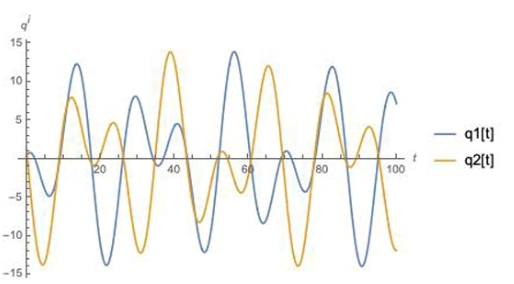
\includegraphics[width=1\textwidth]{/home/tam/Musique/modelRapport(1)/modelRapport/images/graphe.jpg}
	\caption{ces solutions sont tracées en utilisant $\gamma =1$ et les conditions initiales $q^1(0)=1.5 ,\dot{q}^1(0)=-5.1 ,q^2(0)=0.3 ,\dot{q}^2(0)=1$.}
	\label{fig:hannay}
\end{figure}

\subsection{Angle de Hannay}
Comme nous l'avons observé , notre système pourrait \^{e}tre interprété comme un oscillateur de fréquence $A$ monté dans un référentiel non inertiel qui oscille également mais de fréquence $B$ . L'angle de Hannay [15] pourrait \^{e}tre interprété comme un déphasage entre les deux 
oscillateurs .\\ On calcul l'angle de Hannay en considérant le décalage $2\pi+Bt'$ où$ t'$ est le temps qu'il  faut prendre  pour une période du premier oscillateur de fréquence $A$ .Alors 
\begin{equation}
	t'=\frac{2\pi}{A}
\end{equation}
et l'angle de Hannay de notre système est 
\begin{equation}
	\varTheta_H=2\pi+Bt'
\end{equation}
soit 
\begin{equation}
	\varTheta_H=2\pi+2\pi\frac{B}{A}.	
\end{equation}
Par ailleurs, des équations (3.86) et (3.89), nous avons respectivement
$$ C_2=-\frac{\rho\sinh{\gamma}}{\sqrt{\sigma^2-\rho^2}}$$
et \\
$$C_2=-\frac{B}{A}$$
alors 
\begin{equation}
	\frac{B}{A}= -C_2
\end{equation} soit
\begin{equation}
	\frac{B}{A}=\frac{\rho\sinh{\gamma}}{\sqrt{\sigma^2-\rho^2}}. 
\end{equation} En utilisant l'équation (3.126), nous pouvons réécrire l'angle de Hannay sous la forme 
\begin{equation}
	\varTheta_H=2\pi\left(1+\frac{\rho\sinh{\gamma}}{\sqrt{\sigma^2-\rho^2}}\right).	
\end{equation} Pour $\gamma=0$, alors $\varTheta=2\pi$ et cela signifie que les deux oscillateurs sont en phase. Cet angle géométrique dépend des conditions initiales à travers les définitions de $A$ et $B$ évaluées au vecteur de condition initiale correspondant. C'est aussi la conséquence d'un couplage qui peut \^{e}tre interprété comme une dérivée covariante 
\begin{equation}
	Dv^i=\frac{dv^i}{dt}+\frac{C_2}{C_1}\epsilon^{ij}	q^j.
\end{equation}
Alors, nous avons 
\begin{equation}
	Dq^iDq^i=\dot{q}^2+2\frac{C_2}{C_1}\epsilon^{ij}\dot{q}^iq^j+\frac{C^2_2}{C^2_1}q^2	
\end{equation} ce qui implique que 
$$\frac{1}{2}C_1Dq^iDq^i=\frac{1}{2}C_1\left(\dot{q}^2+\frac{C^2_2}{C^2_1}q^2\right)+2C_2 \epsilon^{ij} \dot{q}^iq^j $$ 
soit 
\begin{equation}
	\frac{1}{2}C_1Dq^iDq^i-\frac{1}{2C_1}q^2=\frac{1}{2}C_1\left(\dot{q}^2+\frac{C^2_2-1}{C^2_1}q^2\right)+2C_2 \epsilon^{ij}\dot{q}^iq^j . 	
\end{equation} Par comparaison de cette dernière équation avec l'équation (3.113), la fonction lagrangienne peut \^{e}tre réécrite comme 
\begin{equation}
	L= \frac{1}{2}C_1Dq^iDq^i-\frac{1}{2C_1}q^2
\end{equation}
	
	
	%\section*{Conclusion}
	
	%\chapter*{Conclusions et Perspectives}
	\chapter*{\color{green!30!blue}{Conclusion et Perspectives}}\addcontentsline{toc}{chapter}{Conclusions}
	Nous avons retrouvé la description quantique d'un système non contraint à travers la quantification des variables classiques. La quantification des variables classiques n'est pas suffisant dans le cas des systèmes contraints et nous utilisons la procédure de quantification de Dirac qui  ne peut \^{e}tre directement appliquée lorsque des anomalies de jauge sont présentes . Dans le cas des systèmes avec un nombre de particules variable , nous avons utilisé  la seconde quantification où nous ne faisons aucune quantification supplémentaire, mais elle nous permet de trouver une nouvelle forme de l'hamiltonien du système .\par Nous avons construit un système classique non linéaire , composé de deux oscillateurs couplés. La construction peut \^{e}tre réaliser pour une déformation $\sqrt{T\overline{T}}$ (dans les formalismes lagrangiens et hamiltonien).Le système est intégrable , il possède deux charges conservées en involution $s$ et $j$ , qui sont associées respectivement à la dualité et àn la symétrie de rotation .En considérant les constantes de mouvement $A$ et $B$ (définies en termes de $s$ et $j$) , il est simple d'intégrer l'équation du mouvement en tant que système linéaire .Les constantes $A$ et $B$ sont respectivement les fréquences des deux oscillateurs couplés .Par utilisation des quantités conservées dans l'action , nous avons trouvé comment effectuer la transformation de Legendre de manière plus simple .Il pourrait \^{e}tre intéressant de considérer notre modèle comme une limite non relativiste d'une action , ce domaine de recherche a été abordé par [10,11] dans le contexte des déformations $T\overline{T}$.La carte construite à partir de l'oscillateur harmonique 2D réalise en une seule étape la déformation complète de l'oscillateur harmonique  produit par le mécanisme $T\overline{T}$  .De nombreuses propriétés dynamiques du système étudié ici peut \^{e}tre traduit en ModMax.Enfin , notre système présente également un phénomène de transfert d'énergie et le déphasage entre les deux oscillateurs couplés est appelé angle de Hannay , qui est une propriété géométrique du système .
	
	\chapter*{Références}
		
		\begin{flushleft}
			\begin{enumerate}
				[1] Born, M., \& Infeld, L. (1934). Foundations of the new field theory. Proceedings of the Royal Society of London. Series A, Containing Papers of a Mathematical and Physical Character,
				144(852), 425-451. \par
				[2] Plebanski, J. F. (1987). Lectures on nonlinear electrodynamics (nordita, copenhagen, 1968).Journal of Mathematical Physics, 28, 2171. \par
				[3] Bialynicki-Birula, I. (1983). Nonlinear electrodynamics: Variations on a theme by Born and Infeld. Quantum theory of particles and fields, 31-48. \par
				[4] Bialynicki-Birula, I. (1992). Field theory of photon dust. Acta Physica Polonica. Series B, 23(6), 553-559. \par
				[5] Bandos, I., Lechner, K., Sorokin, D., \& Townsend, P. K. (2020). Nonlinear duality-invariant conformal extension of Maxwell’s equations. Physical Review D, 102(12), 121703. \par
				[6] Kosyakov, B. (2020). Nonlinear electrodynamics with the maximum allowable symmetries. Physics Letters B, 810, 135840. \par
				[7] Babaei-Aghbolagh, H., Velni, K. B., Yekta, D. M., \& Mohammadzadeh, H. (2022).
				Emergence of non-linear electrodynamic theories from T T -like deformations. arXiv preprint arXiv:2202.11156. \par
				[8] Babaei-Aghbolagh, H., Velni, K. B., Yekta, D. M., \& Mohammadzadeh, H. (2022).
				Marginal T T -Like Deformation and ModMax Theories in Two Dimensions. arXiv preprint arXiv:2206.12677. \par
				[9] Ferko, C., Sfondrini, A., Smith, L., \& Tartaglino-Mazzucchelli, G. (2022). Root-T T Deformations. arXiv preprint arXiv:2206.10515. \par
				[10] Rodrı́guez, P., Tempo, D., \& Troncoso, R.√ (2021). Mapping relativistic to ultra/non-relativistic conformal symmetries in 2D and finite $\sqrt{T\overline{T}}$ deformations. Journal of High Energy Physics, 2021(11), 1-15. \par
				[11] Blair, C. D. (2020). Non-relativistic duality and T T deformations. Journal of High Energy Physics, 2020(7), 1-36. \par
				[12] Arnol’d, V. I. (2013). Mathematical methods of classical mechanics (Vol. 60). Springer Science \& Business Media. \par
				[13] Landau, L. D., Lifshitz, E. M., \& Lifšic, E. M. (1960). Mechanics (Vol. 1). CUP Archive. \par 
				[14] Gaillard, M. K., \& Zumino, B. (1981). Duality rotations for interacting fields. Nuclear Physics B, 193(1), 221-244. \par
				[15] Hannay, J. H. (1985). Angle variable holonomy in adiabatic excursion of an integrable Hamiltonian. Journal of Physics A: Mathematical and General, 18(2), 221. \par
				[16] F. Schwabl, Advanced quantum mechanies (QM II) 1997-416 pages.
			\end{enumerate}
		\end{flushleft}
		
	
	%\chapter*{Webographie}
	
	%\chapter*{Annexes}
	
	\newpage
	%\chapter*{\color{green!30!blue}{Table des matières}}
	\renewcommand{\contentsname}{\textcolor{green!30!blue}{Table des matières}}
	\tableofcontents
	%\phantomsection
	\addcontentsline{toc}{chapter}{Table des matières}
	
	%\chapter*{Table des matières}
		
\end{document}